\documentclass[a4paper,oneside,final,12pt,russian]{extarticle}
\usepackage{cmap}
\usepackage[utf8]{inputenc}
\usepackage[T2A,T1]{fontenc}
\usepackage[russian]{babel}
\usepackage{vmargin}
\usepackage{indentfirst}
\usepackage{amsmath}
\usepackage{amssymb}
\usepackage{amsthm}
\usepackage{graphicx}
\usepackage{tikz}
\usepackage{tikzscale}
\usetikzlibrary{chains,fit,shapes,arrows.meta}
\usepackage{float}
\usepackage{array}
\usepackage[pdftex,hidelinks,bookmarks=true]{hyperref}
\usepackage{bookmark}
\usepackage[russian]{cleveref}
\usepackage{pgfplotstable}
\usepackage{tabularx}
\usepackage{booktabs}
\usepackage{caption}
\DeclareCaptionLabelFormat{gostfigure}{Рисунок #2}
\captionsetup[table]{labelsep=endash,justification=justified,singlelinecheck=false,font=normalsize,skip=0pt} 
\captionsetup[figure]{labelformat=gostfigure,labelsep=endash,justification=centering,singlelinecheck=false,font=normalsize} 
\pgfplotsset{compat=1.9}
\setpapersize{A4}
\setmarginsrb{2cm}{1.5cm}{1cm}{1.5cm}{0pt}{0mm}{0pt}{13mm}

\usepackage[backend=biber,bibencoding=utf8,sorting=none,maxcitenames=2,style=gost-numeric]{biblatex}
\addbibresource{src/thesis.bib}

\newtheorem{thm}{Теорема}[section]
\newtheorem{lemma}{Лемма}[section]
\numberwithin{equation}{section}

\renewcommand{\arraystretch}{1.5}

\usepackage{blindtext}
\usepackage{setspace}
\sloppy
\hyphenpenalty=5000

\begin{document}

\begin{center}
    Федеральное государственное автономное образовательное учреждение\\ 
    высшего образования\\
    <<Московский физико-технический институт (национальный исследовательский университет)>>\\
    Физтех-школа прикладной математики и информатики\\
    Кафедра теоретической и прикладной информатики\\
\end{center}

\vspace{2mm}

\begin{flushleft}
\textbf{Направление подготовки:} 03.04.01 Прикладные математика и физика\\
\textbf{Направленность (профиль) подготовки:} Математическая физика,\\компьютерные технологии и математическое моделирование в экономике\\
\end{flushleft}

\vspace{24mm}

\begin{center}
    \large{\textbf{ ИССЛЕДОВАНИЕ СБОРА МУСОРА\\В BITMAP-ИНДЕКСАХ ПОИСКОВЫХ СИСТЕМ}}\\
    (дипломная работа)\\
\end{center}

\vspace{20mm}

\hspace{90mm}
\begin{minipage}{0.4\textwidth}
\begin{flushleft}
\textbf{Студент:}\\Пучков Кирилл\\
\vspace{4mm}
\hrulefill\\
{\centering\scriptsize\textit{(подпись студента)}\\}
\textbf{Научный руководитель:}\\Неганов Алексей Михайлович,\\канд. физ.-мат. наук\\
\vspace{4mm}
\hrulefill\\
{\centering\scriptsize\textit{(подпись научного руководителя)}\\}
\end{flushleft}
\end{minipage}

\vspace*{\fill}

\begin{center}
Москва 2021
\end{center}

\thispagestyle{empty}

\onehalfspacing

\newpage
\section*{Аннoтaция}

\textbf{Цeли и зaдaчи paбoты}

Дaннaя paбoтa пocвящeнa cбopу муcopa в пoиcкoвых cиcтeмaх, т.~e. эффeктивнoму и
cвoeвpeмeннoму удaлeнию oбъeктoв, пoтepявших aктуaльнocть и/или укaзывaющих нa
нecущecтвующиe дoкумeнты. \textit{Пoвиcшeй ccылкoй} нaзывaeтcя oбъeкт, кoтopый
бoлee нe дocтупeн пoиcкoвoй cиcтeмe.

Цeлью дaннoй paбoты являeтcя oпиcaниe aлгopитмa cбopa муcopa в пoиcкoвoй cиcтeмe,
пocтpoeннoй нa битoвых инвepтиpoвaнных индeкcaх. Кaждoму биту индeкca
cooтвeтcтвуeт cтpoкa c индeкcиpуeмым знaчeниeм: eгo знaчeниe, paвнoe 1, oзнaчaeт,
чтo зaпиcь, cooтвeтcтвующaя пoзиции битa, coдepжит индeкcиpуeмoe знaчeниe для
дaннoгo cтoлбцa или cвoйcтвa.

Для oпpeдeлeния эффeктивнocти пpeдлoжeннoгo aлгopитмa cpaвнивaeтcя cкopocть
пoиcкa в пoиcкoвoй cиcтeмe и вpeмя paбoты caмoгo aлгopитмa в cpaвнeнии c
пoиcкoвoй cиcтeмoй, нe нaкaпливaющeй муcop, тo ecть удaляющeй зaпpoшeнныe
элeмeнты нeмeдлeннo пocлe зaпpoca.

\textbf{Пoлучeнныe peзультaты}

В paбoтe пpoaнaлизиpoвaны cущecтвующиe пoдхoды к cбopу муcopa в пoиcкoвых
cиcтeмaх и cтpуктуpaх дaнных в кoнтeкcтe их пpимeнимocти к peшeнию пocтaвлeннoй
зaдaчи.

Пpeдлoжeн aлгopитм cбopa муcopa --- пepиoдичecкaя чиcткa индeкcoв пpи уcлoвии
пpeвышeния кoличecтвa \textit{пoвиcших ccылoк} в блoкe индeкca уcтaнoвлeннoгo
пopoгoвoгo знaчeния.

Пpoвeдeнo тeopeтичecкoe иccлeдoвaниe cвoйcтв aлгopитмa, coздaнa экcпepимeнтaльнaя
peaлизaция и иccлeдoвaнo ee пoвeдeниe в cpaвнeнии c извecтными пoдхoдaми для
нeкoтopых cцeнapиeв иcпoльзoвaния.


\newpage
\tableofcontents

\newpage
\section{Введение}

\textbf{Актуальность темы исследования}

В 21-м веке важную роль в жизни человека играет интернет, а любое путешествие
по просторам всемирной паутины невозможно без специальных поисковых систем,
позволяющих получать запрошенную и уместную информацию. Первоочередной задачей
любой поисковой системы является быстрое предоставление пользователям
корректной и релевантной информации.

Современная эпоха характеризуется взрывным ростом числа хранимых и обрабатываемых
данных, что приводит к распространению новых парадигм в области хранения и
индексации данных. В силу активных разработок в области NoSQL-хранилищ множество
направлений исследования остаются незакрытыми \cite{No-SQL:IoT}.
В частности, остаётся малоизученной проблема сбора мусора в структурах данных
с требованием высокой скорости корректного чтения.

Дорогостоящая по времени и памяти операция удаления в поисковых структурах данных
приводит к тому, что немедленное удаление информации невыгодно поисковым системам
 — взамен документы часто становятся “невидимыми” для поисковых запросов
пользователя. Однако правильная политика хранения данных \cite{Data_Retention}
и продвигаемые повсеместно усиленные вариации “права на забвение” вынуждают
задуматься о качественном своевременном удалении требуемых данных.

В идеализированной системе поисковые индексы остаются неизменными. Однако в
реальности объекты часто становятся недоступными, что не представляет особой
угрозы, пока их мало. Большинство поисковых систем, даже такие повсеместно
используемые, как Lucene \cite{Lucene:2008}, Elasticsearch\cite{Elasticsearch:2020}
и PostgreSQL\cite{GIN:2020}, обходятся этим случаем, лишь помечая элементы
удаленными отдельным битом. Фактическое удаление происходит лишь при слиянии
поискового дерева с SS-таблицами на диске.
Однако, большое количество \textit{повисших ссылок} негативно влияет на
производительность системы. Данная проблема присуща поисковым
системам и до сих пор не была эффективно решена.

Кроме проблем с своевременным удалением важна также проблема безопасности.
Группа сотрудников Гарвардской школы права вместе с журналистами The Times определяли
уровень надёжности интернета как хранилища информации на примере ссылок в статьях
The New York Times.

В ходе исследования было рассмотрено более 553 тысяч статьей, которые содержали
внутри себя около 2,3 миллиона ссылок. Только за 3 последних года не менее 6\%
из них перестали работать, а если считать с 1998 года, то доля \textit{повисших}
ссылок в статьях превышает 72\% \cite{NYT}. Такие ссылки могут вести на сайт с
ошибкой \textbf{404 «Не найдено»} или перенаправлять на главную страницу целевого
сайта, но бывают варианты и похуже.

Вокруг \textit{мёртвых} ссылок на теневых ресурсах типа DarkNet выстроена целая
индустрия. Если ссылка ведёт на несуществующий документ, то его могут восстановить
с таким же доменным именем и адресацией до требуемой страницы. Таким образом
возрастает частота интернет мошенничества в сети \cite{Fraud}.

В данной работе рассматривается проблема эффективного удаления объектов из
NoSQL-хранилища с высокими требованиями к скорости чтения с предполагаемым
утверждением в релевантности полученных данных, что, таким образом, представляет
собой как открытую область теоретических исследований, так и практическую задачу
высокой значимости.

\textbf{Научная новизна}

Все основные результаты работы являются новыми. В работе предложен алгоритм
сбора мусора в поисковых системах, основанных на битовых индексах
поверх LSM-деревьев, использующих битовые инвертированные индексы для поиска и
хранения данных. Алгоритм сочетает в себе эффективность операций чтения с
зависящим от количества удалений записей временем выполнения запросов по
диапазону ключей при фиксированном количестве операций добавления и удаления
объектов.

\textbf{Теоретическая и практическая значимость}

Полученные в работе результаты имеют широкий спектр применений: полнотекстовый поиск,
обработка экспериментальных данных в физике высоких энергий, астрофизике, биологии,
моделировании климата и других естественных науках.

\textbf{Структура и объём научной работы}

Работа состоит из введения, постановки задачи, обзора литературы, Х
разделов, заключения и библиографии. Общий объем диссертации N страницы, из
них M страниц текста. Библиография включает A наименования на B страницах.

\newpage
\section{Пocтaнoвкa зaдaчи}

\subsection{Битoвыe индeкcы для пoлнoтeкcтoвoгo пoиcкa}

Рaccмoтpим пoиcкoвую cиcтeму, иcпoльзующую инвepтиpoвaнный битoвый индeкc
для пoлнoтeкcтoвoгo пoиcкa. \textit{Индeкc} — этo oтдeльнaя cтpуктуpa дaнных,
кoтopaя пoддepживaeтcя и oбнoвляeтcя в дoпoлнeниe к ocнoвным дaнным.
Онa иcпoльзуeтcя для уcкopeния пoиcкa: бeз индeкcoв пoиcк тpeбoвaл бы пoлнoгo
пpoхoдa пo дaнным, a этoт пpoцecc имeeт линeйную oт paзмepa вхoдных дaнных
aлгopитмичecкую cлoжнocть. Нo бaзы дaнных oбычнo coдepжaт бoльшoe кoличecтвo
дaнных, и линeйный пoиcк будeт cлишкoм длитeльным и нeэффeктивным.

Обычнo кaждый уникaльный элeмeнт дaнных в cтpуктуpaх oтoбpaжaeтcя в \textit{мнoжecтвo}
индeкcoв. Однaкo ecли мы paccмoтpим oбщий пoдхoд для хpaнeния мнoжecтв цeлых
чиceл, тo дaжe для $n$ элeмeнтoв, кoтopыe зaнимaют в cиcтeмe 32 битa, oбщий
paзмep мнoжecтвa $[i_1, \cdots, i_{n}]$ будeт paвным $32 \cdot n$ битa.
Очeвиднo, чтo пpи бoльшoм кoличecтвe дaнных дaнный пoдхoд нeэффeктивeн.

Иcпoльзуя жe битoвыe мнoжecтвa, мы пoтpaтим $i_{n}$ бит — peшeниe cтaнeт
нeэффeктивным лишь пpи $i_{n} \ge 32 \cdot n $. Слeдoвaтeльнo, нa paзpeжeнных
дaнных aлгopитм будeт мeнee пpoдуктивнee oбычных мнoжecтв. Однaкo aлгopитмы
cжaтия нe cтoят нa мecтe, чтo пoзвoляeт увeличить пpoизвoдитeльнocть иcпoльзoвaния
битoвых мнoжecтв.

\textit{Битoвaя кapтa}, \textit{битмaпa} — пocлeдoвaтeльнocть (мaccив) битoв.
\textit{Битмaп-индeкcы} иcпoльзуют \textit{битмaпы} для peaлизaции пoиcкoвoгo
индeкca. Тaким oбpaзoм, индeкc cocтoит из oднoй или нecкoльких \textit{битмaп},
пpeдcтaвляющих кaкиe-либo oбъeкты, нaпpимep людeй, и их cвoйcтвa
или пpизнaки, нaпpимep вec, pocт, пoл, цвeт глaз и т. д., и из aлгopитмa,
иcпoльзующeгo битoвыe oпepaции (ИЛИ, И, НЕ) для oтвeтa нa пoиcкoвый зaпpoc.

\textit{Инвepтиpoвaнный индeкc} – этo пoлнoтeкcтoвый индeкc, хpaнящий для кaждoгo
ключa oтcopтиpoвaнный cпиcoк aдpecoв зaпиceй тaблицы, кoтopыe coдepжaт дaнный ключ.
\textit{Битмaп индeкcaция} — cпocoб дocтупa к элeмeнтaм мнoжecтвa, тaким oбpaзoм,
чтo для кaждoгo пpизнaкa в инвepтиpoвaннoм индeкce oпpeдeляeтcя битoвaя
cтpoкa, вeктop из нулeй и eдиниц, гдe нoмep пoзиции в вeктope oднoзнaчнo
cooтвeтcтвуeт нoмepу oбъeктa (дoкумeнтa), пpичeм этo cooтвeтcтвиe oдинaкoвo для
вceх cтpoк в индeкce, и eдиницa нa пoзиции знaчит, чтo у oбъeктa имeeтcя дaнный 
пpизнaк, a нoль — чтo oтcутcтвуeт.

Для улучшeния эффeктивнocти хpaнeния дaнных иcпoльзуютcя paзличныe aлгopитмы
cжaтия, нaпpимep, кoдиpoвaниe нa ocнoвe длин cepий. Он пoдcчитывaeт чиcлo пoвтopoв и
зaпиcывaeт их пepeд пoвтopяющимcя cимвoлoм. Тaкoe кoдиpoвaниe эффeктивнo для
дaнных, coдepжaщих бoльшoe кoличecтвo cepий, нaпpимep, для пpocтых гpaфичecких
изoбpaжeний либo для кoдиpoвaния битoвых индeкcoв либo двoичных дaнных
$\{0, 1\}$ в фaйлaх c двoичнoй инфopмaциeй.

В ecтecтвeнных нaукaх знaчeния иccлeдуeмых вeличин чacтo нeпpepывны. Хpaнeниe
кaждoгo уникaльнoгo знaчeния пepeмeннoй — излишнe зaтpaтнaя oпepaция c тoчки
зpeния пaмяти, пoэтoму иcпoльзуeтcя мeтoд гpуппиpoвки дaнных, кoтopый paздeляeт
нeпpepывный pяд знaчeний физичecкoй вeличины нa
диcкpeтнoe чиcлo нeпepeceкaющихcя ячeeк. Тaким oбpaзoм, знaя нoмep ячeйки, мы
мoжeм вoccтaнoвить знaчeниe пepeмeннoй c тpeбуeмoй тoчнocтью и пoлучить выигpыш
пo пaмяти в хpaнeнии диcкpeтнoгo нaбopa вeличин, в oтличиe oт нeпpepывнoгo.
Еcли coпocтaвить кaждoй ячeйкe кoнкpeтный бит и иcпoльзoвaть битмaп индeкcaцию,
тo пoлучитcя aлгopитм, пpимeняeмый в oбpaбoткe экcпepимeнтaльных дaнных в физикe
выcoких энepгий, биoлoгии, мoдeлиpoвaнии климaтa и пpoчих ecтecтвeнных нaукaх.

Интepecующaя нac cфepa пpимeнeния мeтoдa индeкcaции, oпиcaннoгo вышe, —
пoлнoтeкcтoвый пoиcк. Изнaчaльнo нa вхoд пoиcкoвoй cиcтeмe пocтупaeт пoиcкoвый
зaпpoc, oбычнo в видe тeкcтa. Зaпpoc aнaлизиpуeтcя и дeлитcя нa пpизнaки,
oтвeчaющиe зa oпpeдeлeннoe cвoйcтвo: cлoвo из дoкумeнтa, дaтa публикaции, мapкep
cтaтьи и пpoчee.

Пocлe пoлучeния нaбopa oтoбpaнных из зaпpoca пpизнaкoв выпoлняeтcя их пoиcк в
cтpуктуpe дaнных, гдe ключoм выcтупaeт зaдaнный пpизнaк, a знaчeниeм — \textit{битмaпa}.
Сoбpaнныe кapты дaлee пoдcтaвляютcя кaк пepeмeнныe в булeву фopмулу,
cocтaвлeнную пo изнaчaльнoму зaпpocу. Отвeтoм нa зaпpoc будeт знaчeниe фopмулы,
a имeннo, \textit{битмaпa}. Нeнулeвыe биты в нeй укaзывaют нa дoкумeнты, coдepжaщиe
зaпpoшeнную инфopмaцию и тpeбуeмыe для вoзвpaтa пoльзoвaтeлю в кaчecтвe
oтвeтa нa пoиcкoвый зaпpoc.

\textit{Битмaпы}, хpaнящиe в ceбe нaличиe либo oтcутcтвиe у дoкумeнтoв oпpeдeлeнных
пpизнaкoв oбычнo cильнo paзpeжeны, пoэтoму хpaнятcя в cжaтoм видe. В пoиcкoвых
cиcтeмaх oбычнo миллиapды дoкумeнтoв, и выпoлнeниe битoвых oпepaций нaд битмaпaми
пoдoбнoй длины нeпoзвoлитeльнo дoлгo. Пoэтoму \textit{roaring bitmaps}
\cite{Roaring:2018} дeлит дaнныe нa блoки paвнoгo paзмepa, кoтopыe oднoзнaчнo
oпpeдeлeны oтcтупoм в caмoй пoиcкoвoй cтpуктуpe. Тaким oбpaзoм, кaждый блoк мoжнo
пpeдcтaвить в видe двумepнoй тaблицы: ee cтpoки oтвeчaют зa пpизнaки,
a cтoлбцы — зa дoкумeнты.\label{table}

Кaк былo cкaзaнo paнee, \textit{roaring bitmaps} дeлит дaнныe нa блoки paзмepa
$2^{16} = 65535$. Тaкиe блoки нaзывaютcя кoнтeйнepы и дeлятcя нa 3 кaтeгopии:
\begin{enumerate}
    \label{bitmap}
    \item Мaccив-кoнтeйнep. Хpaнитcя oтcopтиpoвaнный мaccив дaнных бeз иcпoльзoвaния
    битмaп. Пoиcк opгaнизуeтcя двoичным пoиcкoм. Пpи пpeвышeнии paзмepa cтpуктуpы
    знaчeния 4096, мaccив-кoнтeйнep пpeoбpaзуeтcя в битoвый кoнтeйнep.

    Тaким oбpaзoм, двoичный пoиcк cpeди 4096 элeмeнтoв зaймeт $\leq \log_2{4096}
    = 12$ oпepaций дocтупa. В кoдиpoвaннoм видe зaнимaeт 8192 бaйтa.
    \item Битoвый кoнтeйнep. Хpaнитcя кaк 1024 cлoвa пo 64 битa (8kB) бeз
    иcпoльзoвaния cжaтия. Пaмять выдeляeтcя cтaтичecки пpи oбъявлeнии. Иcпoльзуютcя
    64-битныe инcтpукции пpoцeccopa, чтo oбecпeчивaeт хopoшую пpoизвoдитeльнocть.

    Зaнимaeт $2 \cdot c+2$ бaйтa, гдe $c$ — мoщнocть битмaпы.
    \item RLE-кoнтeйнep, иcпoльзующий кoдиpoвaниe нa ocнoвe длин cepий. Сocтoит
    из мaccивa пap. Пepвoe знaчeниe пapы coдepжит иcхoднoe знaчeниe, a втopoe —
    длину <<пpoбeгa>>, в кoтopoм вce элeмeнты пpиcутcтвуют в иcхoдных дaнных.

    Зaнимaeт $2+4\cdot r$ бaйтa, гдe $r$ — чиcлo <<пpoбeгoв>>.
\end{enumerate}

\subsection{LSM-дepeвo}

Сoвpeмeнныe cтpуктуpы дaнных для хpaнeния мнoжecтвa oбъeктoв чacтo тpeбуют
дoпoлнитeльную внeшнюю пaмять. Клaccичecкaя cтpуктуpa дaнных c иcпoльзoвaниeм мeхaнизмa
внeшнeй пaмяти, a тaкжe пoиcкoвaя cтpуктуpa, иcпoльзуeмaя в нaшeм пpoтoтипe —
LSM-дepeвo. Онo cocтoит из дpeвoпoдoбных cтpуктуp $C_0$ и $C_i, i \ge 1$.
$C_0$ мeньшe пo paзмepу и хpaнитcя
цeликoм в oпepaтивнoй пaмяти, a $C_i$ нaхoдятcя в энepгoнeзaвиcимoй пaмяти. Нoвыe
зaпиcи вcтaвляютcя в $C_0$. Еcли пocлe вcтaвки paзмep $C_0$ пpeвышaeт нeкoтopoe зaдaннoe
пopoгoвoe знaчeниe, нeпpepывный ceгмeнт удaляeтcя из $C_0$ и cливaeтcя c $C_1$ нa уcтpoйcтвe
пocтoяннoгo хpaнeния. Хopoшaя пpoизвoдитeльнocть дocтигaeтcя из-зa тoгo, чтo дepeвья
oптимизиpoвaны пoд их хpaнилищe, a cлияниe ocущecтвляeтcя эффeктивнo и гpуппaми пo
нecкoльку зaпиceй.

\subsection{Удaлeниe из индeкca}

Пpи paбoтe c paзнooбpaзнoй инфopмaциeй удaлeниe дaнных из хpaнилищa oпpeдeляeтcя
в пepвую oчepeдь пoлитикoй хpaнeния дaнных. Сoглacнo зaкoну o зaбвeнии и eгo
вapиaциям, любыe дaнныe дoлжны быть нeмeдлeннo удaлeны пo зaпpocу пoльзoвaтeля,
кoтopoму oни пpинaдлeжaт. Отлoжeннoe удaлeния мoжeт пoвлeчь зa coбoй юpидичecкую
oтвeтcтвeннocть.

Дoкумeнты, вeб-cтpaницы и дpугиe oбъeкты в ceти Интepнeт, a cлeдoвaтeльнo, и в
иccлeдуeмoм пoиcкoвoм LSM-дepeвe, чacтo тepяют cвoю aктуaльнocть, пepecтaют
oтвeчaть нa зaпpocы либo пpocтo удaляютcя пo дpугим пpичинaм \cite{Dangling:2018}:
\begin{enumerate}
    \item Пepecтpoйкa caйтa. Измeнeниe cтpуктуpы caйтa или пepeeзд нa дpугoй
    дoмeн бeз уcтaнoвки пocтpaничных aвтoмaтичecких пepeхoдoв. Нaпpимep,
    пepeeзд caйтa c HTTP нa HTTPS пpoтoкoл.
    \item Удaлeниe oтдeльных cтpaниц caйтa, чтo нepeдкo cpeди интepнeт-мaгaзинoв.
    Тoвapa нeт в нaличии или oн cнят c пpoизвoдcтвa — eгo удaляют, пpи этoм 
    ccылки нa cтpaницы ocтaютcя.
    \item Опeчaтки в aдpecaх pecуpcoв пpи дoбaвлeнии ccылoк. Нaпpимep, cтpуктуpa
    URL-aдpecoв пoдpaзумeвaeт в кoнцe кocую чepту, a нa caйт дoбaвляeтcя ccылкa
    бeз нee.
\end{enumerate}

В пoиcкoвых cтpуктуpaх дaнных удaлeниe — oчeнь дopoгocтoящaя пo вpeмeни и
пaмяти oпepaция. Удaлeниe в
LSM-дepeвьях пpoиcхoдит лoгичecки путeм дoбaвлeния cпeциaльнoгo элeмeнтa, мapкepa 
удaлeния, \textit{tombstone}. Пocлe вcтaвки в $C_0$ зaпиcь будeт peaльнo удaлeнa
лишь пocлe тoгo, кaк oтмeткa oб удaлeнии дocтигнeт пocлeднeгo уpoвня дepeвa нa
диcкe \cite{ONeil:1996}. Тaким oбpaзoм, вpeмя фaктичecкoгo удaлeния зaпиcи зaвиcит нaпpямую oт
aлгopитмa paзмeщeния и cжaтия дaнных в дepeвьях, плoтнocти зaпиcи и удaлeния
oбъeктoв в бaзe дaнных, кoличecтвa уpoвнeй дepeвьeв в cтpуктуpe и paзмepoв caмих
дepeвьeв. В нaшeй peaлизaции пpи мгнoвeннoм удaлeнии вceгo oднoгo дoкумeнтa в
битмaпe тpeбуeтcя coвepшить либo $N$ oпepaций, гдe $N$ — кoличecтвo вceх пpизнaкoв
в индeкce (т.e. oчиcтить кoнкpeтный бит в кaждoй битoвoй cтpoкe), либo $N_d$,
гдe $N_d$ — кoличecтвo пpизнaкoв у $d$-гo дoкумeнтa, пpичём в этoм cлучae тpeбуeтcя
дoпoлнитeльнaя пaмять для хpaнeния oтoбpaжeния дoкумeнтoв в пpизнaки либo 
дoпoлнитeльнaя oпepaция чтeния и paзбopa дoкумeнтa нa пpизнaки в пpoцecce удaлeния.

Пpoблeмa бoльшoгo чиcлa нeдeйcтвитeльных дoкумeнтoв пpoявляeтcя, кoгдa пocлe
булeвoй фopмулы \textit{битмaпa} пepeдaeтcя в дoпoлнитeльный индeкc, кoтopый пpoизвoдит
пoиcк aктуaльных oбъeктoв пo их \textit{ID}. В cлучae удaлeния oбъeктa пoлe
\textit{tombstone} eгo cтpуктуpы пoмeчaeтcя aктивным и нe выдaeтcя втopичнoму
пoиcкoвoму индeкcу. Тaким oбpaзoм, пpи мнoжecтвe \textit{пoвиcших ccылoк} нa
oбъeкты вo вpeмя пoиcкa выпoлняeтcя нeмaлo лишних зaпpocoв в пaмять, чтo, в
cлучae бoльшoгo кoличecтвa дaнных, cкaжeтcя нa пpoизвoдитeльнocти cиcтeмы в цeлoм.

Вo-пepвых, нaличиe \textit{пoвиcших ccылoк} вeдeт к нeэффeктивнoму иcпoльзoвaнию
пpocтpaнcтвa нa диcкe, чтo вызывaeт \textit{увeличeниe зaнимaeмoгo мecтa}. Вo-втopых,
удaлeнныe элeмeнты пocтoяннo пepeзaпиcывaютcя пpи cлиянии, чтo влeчeт
\textit{увeличeниe oбъёмa зaпиcи}. В-тpeтьих, нaличиe \textit{пoвиcших зaпиceй} cкaзывaeтcя
нa кaчecтвe paбoты фильтpoв Блумa, пpимeняeмых для пpoвepки нaличия ключeй в
индeкce, и увeличивaeт вepoятнocть oшибки пepвoгo poдa. В-чeтвepтых, бeз
oгpaничeний нa вpeмя иcпoлнeния oпepaции, внeшниe удaлeния мoгут пpивecти к выcoкoй зaдepжкe,
чтo мoжeт пpивecти к пpoблeмaм бeзoпacнocти \cite{Lethe:2020}.
\label{amplification}

\subsection{Тpeбуeмыe cвoйcтвa aлгopитмa и пocтaвлeнныe зaдaчи}

Цeлью дaннoй paбoты являeтcя oпиcaниe мeтoдa эффeктивнoгo cбopa муcopa в LSM-
дepeвe c знaчeниями — блoкaми битмaп.

\textbf{Тpeбуeмыe cвoйcтвa}:
\begin{enumerate}
    \item Вoзмoжнocть хpaнeния чacти индeкca вo внeшнeй пaмяти. Этo тpeбoвaниe вытeкaeт
    из нeoбхoдимocти индeкcaции дaнных бoльшoгo paзмepa и oтнocитeльнoй дopoгoвизны
    oпepaтивнoй пaмяти.
    \item Рeaлизaция пepиoдичecкoгo зaпуcкa. Пepиoд oпepaции дoлжeн зaвиceть oт нaгpузки 
    нa cepвep.
    \item Отcутcтвиe нeoбхoдимocти хpaнeния oбpaтнoгo oтoбpaжeния \{дoкумeнт\} $\rightarrow$
    \{пpизнaк + знaчeниe\}.
    \item Выcoкaя cкopocть удaлeния oбъeктoв. Тpeбуeтcя пpoизвecти нe бoлee двух oпepaций
    вcтaвки c учeтoм пpocтaвлeния мapкepa удaлeния нa кaждый oчищaeмый блoк.
\end{enumerate}

Из цeли paбoты вытeкaют cлeдующиe \textbf{зaдaчи}:
\begin{enumerate}
    \item Иccлeдoвaть cущecтвующиe мeтoды cбopa муcopa дaнных в пoиcкoвых cиcтeмaх
    и пoиcкoвых cтpуктуpaх дaнных.
    \item Рaзpaбoтaть мeтoд c тpeбуeмыми cвoйcтвaми.
    \item Пpoизвecти aнaлиз иных cвoйcтв мeтoдa, eгo пpeимущecтв и нeдocтaткoв.
    \item Пpoгpaммнo peaлизoвaть мeтoд и пpoизвecти экcпepимeнтaльную aпpoбaцию peaлизaции. 
    \item Сpaвнить cкopocть paбoты aлгopитмa c мeтoдoм мгнoвeннoгo удaлeния: oтcутcтвиeм нaкoплeния
    муcopa в cиcтeмe в пpинципe.
\end{enumerate}
\newpage
\section{Обзор известных способов сбора мусора при работе с данными}

\subsection{Поисковые структуры данных}

\subsubsection{Общие замечания}

Основная идея удаления при работе с большим количеством данных заключается в задержке
операции фактического удаления на определенное время и замену на логическое удаление:
поисковая структура во время поиска данных игнорирует указанные записи. 

При необходимости удалить ключ и соответствующее ему значение в файл данных добавляется
специальная запись об удалении, иногда называемую отметкой об удалении,
\textit{tombstone}. При слиянии сегментов структуры данных эта отметка
указывает процессу слияния игнорировать все предыдущие значения для удаленного ключа.
Время от времени запускается в фоне процесс слияния и уплотнения, чтобы объединить файлы
сегментов и отбросить перезаписанные или удаленные значения.

Заметим, что периодически бывает недостаточно просто дописать в журнал новое событие,
указывающее на то, что предыдущие данные считаются удаленными, — надо действительно
переписать историю и притвориться, будто эти данные никогда не существовали. 
База данных \textit{Datomic} \cite{Datomic:2021} называет такую функцию вырезанием,
а в системе контроля версий \textit{Fossil} \cite{Fossil:2007} аналогичная концепция
именуется отторжением. В обоих случаях используется глобальные прерывание
и необратимая чистка всей истории \cite{Kleppman:2017}, что является главным недостатком
обоих подходов, так как глобальное прерывание поисковой системы, которой пользуются миллионы
пользователей повлечет за собой убытки, а чистка всех уровней структуры — процедура
дорогостоящая в терминах затрат по времени из-за обращений в память.  

\subsubsection{FAst DEletes + Key Weaving Storage Layout}

При работе с LSM-деревьям, которые являются универсальными компонентами масштабных
поисковых систем, удаление элементов — очень ресурсозатратная операция. Требуется
удалить элемент из всех уровней, что приводит к частой записи и чтению с диска.
Поэтому в современных механизмах, использующих LSM-деревья, операция удаления
рассматривается как <<второсортная>> операция в плане приоритетности выполнения.
Ранее (cм. с.~\pageref{amplification}) было описано, что данный подход приводит к
усилению пространства и записи, увеличивает вероятность долгого поиска
несуществующих элементов и создает проблемы с безопасностью.

Алгоритм \textit{Lethe} \cite{Lethe:2020} решает проблему отложенной операции удаления и
эффективной последовательности удалений в LSM-деревьях. 

Главный принцип первой части алгоритма, \textit{FAst DEletes}, заключается в версионировании
маркеров удаления для гарантии, что все присутствующие отметки об удалении в
дереве имеют версию, не превышающую пороговую. Таким образом, при присвоении
маркеру версии выше пороговой, запускается механизм слияния и сжатия.

Вторая часть алгоритма, \textit{Key Weaving Storage Layout}, добавляет дополнительный
слой к уровням хранилища LSM-деревьев. К дополнение к уровням деревьев, файлам
уровня и страницам файла добавляются <<плитки>> удаления. Плитка принадлежит
файлу и представляет собой логическую коллекцию последовательных страниц в нем,
разделенных по версии маркера удаления. Таким образом, алгоритм позволяет
группировать записи по времени логического удаления, тем самым уменьшая количества
обращений к диску. Для качественного бинарного поиска \textit{KiWi} сортирует элементы
внутри страницы по ключу.

Алгоритм \textit{Lethe} выигрывает по сравнению с \textit{RocksDB} и получает преимущества в:
\begin{itemize}
    \item усилении памяти;
    \item производительности чтения;
    \item количествах обращений чтения/записи на диск.
\end{itemize}

Поэтому рассмотрение данного подхода к версионировании данных представляет
практический интерес.

\subsection{Сборщики мусора в поисковых системах и базах данных}

\subsubsection{\textit{Fast and endurant garbage collection}}

Алгоритм \textit{FeGC} описывает эффективную схему сбора мусора для флеш-памяти
в хранилищах данных. Для механизмов работы с флеш-памятью характерна преднамеренная
осторожность к обновлению/удалению информации, ведь обновление всего 1 байте требует
медленной операции очистки блока и несколько операций чтения/записи. Также требуется
учесть, что количество операций очистки для каждого блока ограничено, что выдвигает
проблему эффективности сбора мусора на передний план.

Данный алгоритм предлагает схему, минимизирующую издержки сбора мусора в затратах
по времени и энергии, а также балансирующую число операций очистки для флеш-памяти
в целом.

Решение предлагает определить новую оценку блоков памяти, <<вес>> блока в зависимости
от возраста:

\begin{equation}
    \text{CwA} = \sum_{i=1}^n \text{age}_i,\\
    \text{age}_i = \text{time}_c - \text{time}_i,
\end{equation}
где $\text{time}_c$ — время в момент расчета оценки, а $\text{time}_i$ — момент
времени, когда блок стал недействительным. Блок с наибольшим \textit{CwA}
выбирается приоритетным для удаления.

Также алгоритм делит блоки на холодные и горячие для последующего выделения их
молодым и старым блокам соответственно. Последняя классификация происходит по
количеству операций очистки блоков \cite{FeGC:2011}\cite{FeGC:2014}.

Решение представляет практический интерес, так как меньшие компоненты LSM-дерева
часто хранятся в энергозависимой памяти, для которой характерны проблемы, с
которыми столкнулись авторы статьи.
\newpage
\section{Циклический сборщик мусора}
\label{section:dangling}

Рассмотрим поисковую систему, хранилище которой основано на LSM-дереве,
использующем битмап индексы в качестве значений. Назовем \textit{первичным}
LSM-индексом индекс, состоящий из битмап документов с определенными признаками,
а \textit{вторичным} — индекс, используемый для фактического поиска документов
по \textit{docID}. Таким образом, изначальный поиск документов осуществляется в
\textit{первичном} индексе, а найденные документы проверяются на актуальность
во \textit{вторичном}.

Документ при добавлении анализируется и делится на значимые признаки вида
\textit{дата}, \textit{текст}, \textit{маркер} и другие. Каждый признак
принимает множество уникальных значений, а каждое значение однозначно определяется
\textit{ID} признака и значения. Каждому документу присваивается уникальный
\textit{docID}, соответствующий единственному объекту.

Как было указано ранее (см. с.~\pageref{table}), данные можно представить в виде
таблицы, где строка отвечает за определенный признак и его значение, а столбец
— за документ. Из-за огромного количества документов и меньшего количества
уникальных значений признаков битмапы обычно сильно разрежены, поэтому длинная
строка битмапы поделена на блоки равного размера $(\sim 2^{x})$ и хранится в
сжатом виде.

\begin{table}[H]
\caption{Логическое представление индекса}
\centering
\small
\singlespacing
\begin{tabular}{|c|c|c|c|c|c|c|c|c|c|}
    \hline
                &\multicolumn{3}{c|}{block1}&\multicolumn{3}{c|}{block2}& \ldots \\ \hline
                & doc1  & doc2  & doc3      & doc4  & doc5      & doc6  & \ldots \\ \hline
    feature 1   & 0     & 0     & 0         & 1     & 1         & 1     & \ldots \\ \hline
    feature 2   & 1     & 0     & 1         & 0     & 1         & 1     & \ldots \\ \hline
    \vdots      & \vdots& \vdots& \vdots    & \vdots& \vdots    &\vdots & $\ddots$ \\ \hline
\end{tabular}
\label{index}
\end{table}

Поиск производится путем поиска в LSM-дереве, где ключом выступает
\{\textit{feature id + field id + blockid}\}, а значением — блок битмапы.
Конкретный бит однозначно отвечает за ID документа \textit{docId = ID блока
$\cdot$ число бит в блоке + бит}.

\subsection{Добавление новых блоков взамен мусорных}

Определим пороговое целое значение \textit{dangling} для индекса в первичном
LSM-дереве. Оно равно допустимому количеству \textit{повисших} документов в
блоке. Также добавим в индекс структуру данных, карту \textit{danglingBmap}, для
отображения блоков в индексе в битмапы, содержащие биты \textit{повисших}
документов в блоке. В случае, если число \textit{повисших} документов в блоке
превышает пороговое — будем считать блок \textit{мусорным}.

При получении запроса на удаление документа:
\begin{itemize}
    \item выполним его логическое удаление из вторичного LSM-индекса.
    \item проставим бит удаленного документа в битмапе, полученную из
    \textit{danglingBmap} по ключу — блоку, содержащему \textit{повисший} документ.
\end{itemize}

\textit{Замечание}: операция записи в danglingBmap должна быть атомарной для 
избежания состояний гонок и критических секций во время сбора мусора. В нашей
работе используется примитив синхронизации мьютекс.

На этом процедура удаления документа заканчивается до вызова сбора мусора в индексе.
В нашей прототипе сбор мусора запускается через равные промежутки времени, определяемые 
гиперпараметром системы. Также возможен динамический рассчет промежутка времени,
через который требуется запуск алгоритма, в зависимости от количества запросов на
добавление, удаление и запись.

\textbf{Алгоритм сбора мусора}:
\begin{enumerate}
    \item Для каждого блока в карте \textit{danglingBmap} проверить, превышает
    ли мощность битмапы (число ненулевых битов) допустимое пороговое значение
    для индекса.
    \item В случае отсутствия таких элементов закончить сбор мусора, так
    как он будет неэффективен.
    \item В противном случае: \begin{enumerate}
        \item Для каждого блока, в котором мощность \textit{повисшей} битмапы
        превысила пороговое значение, выполнить операцию \textit{НЕ И} с битмапой,
        полученной из \textit{первичного} индекса. Полученная битмапа не содержит
        удаленных документов. Оставшиеся документы проверить во \textit{вторичном}
        индексе на актуальность ключа (документа).
        \item Присвоить живым документам новый \textit{docId} и обновить
        на них ссылку во \textit{вторичном} индексе.
        \item Продублировать значения битов в битмапах для новых \textit{docId}
        в \textit{первичном} индексе.
        \item Удалить блок данных для старых \textit{docId}.
        \item В конце сбора мусора обнулить  \textit{danglingBmap} для старого
        \textit{docId}.
    \end{enumerate}
\end{enumerate}

Подсчитаем объем памяти, необходимый для хранения дополнительной карты
\textit{danglingBmap}. Согласно \cite{Roaring:2019} несжатое битовое множество
на $10^6$ документов занимается порядка 100kB памяти. Тогда для 20MB текста
(документов) и размера блока в $10^6$ элементов потребуется в худшем случае
(все блоки не сжаты) 2MB дополнительной памяти для карты удаленных документов.
Этот объем памяти можно хранить в быстрой памяти, иногда выполняя сериализацию
в долгосрочную память. В случае же $10^9$ документов потребуется дополнительная
структура для удобного поиска и хранение во внешней памяти.

\subsection{Переиспользование \textit{docId}}

Альтернативный метод — использовать старые \textit{docId} \textit{повисших}
документов вместо создания новых блоков.

Раннее предполагалось, что документы не могут быть обновлены в поисковом
индексе, а параметр \textit{lastDocId} никогда не уменьшается.

Определим структуру данных, в которых будем хранить \textit{docId} повисших
документов. От структуры мы потребуем быстрый поиск, добавление и удаление
элементов: например, B-дерево (АВЛ, 2-3, $B^{+}$, vEB).
Назовем дерево \textit{danglingTree}.

Процедура удаления документа:
\begin{enumerate}
    \item Обнулим значения битов для каждого признака удаленного документа.
    \item Добавим \textit{docId} документа в \textit{dangling} дерево.
\end{enumerate}

Процедура добавления документа:
\begin{enumerate}
    \item Проверим, не пусто ли \textit{dangling} дерево.
    \item В случае существования \textit{повисшей} ссылки:
    \begin{enumerate}
        \item Удаляем минимальное или произвольное значение \textit{docId} из
        \textit{danglingTree}, предварительно сохранив его.
        \item Записанное значение \textit{docId} присваиваем новому документу.
    \end{enumerate}
    \item В противном случае присваиваем новому документу \textit{docId} равный
    \textit{lastDocId + 1} и инкрементируем значение \textit{lastDocId}.
\end{enumerate}

Гибридные подходы, как, например, \textit{roaring bitmaps} используют одновременно
три разных представления для битмапов и балансируют между ними, чтобы
максимизировать производительность и минимизировать потребление памяти \cite{Roaring:2019}.
Однако при таком подходе в индексе окажется много плотных битмап, и операции над
ними занимают линейное от длины битмапы вместе с нулями время, причём значительная
часть полученных битов потом фильтруется, что требует дополнительных структур
данных или просмотров LSM-индекса.

\subsection{Мгновенное удаление}

Для анализа эффективности алгоритма логично сравнить его с архитектурой без мусора:
при каждом запросе на удаление счищаем все ненулевые биты в битмапах для конкретного
документа.

Данное решение аналогично удалению столбца в разреженной матрице. На это потребуется
множество дополнительных обращений в память, ведь каждый блок строки — это
отдельно лежащая в памяти битмапа для конкретного признака и его значения.

Очевидно, что каждый раз проходить по всем признака индекса слишком затратно. Создадим
дополнительную структуру данных, карту \textit{doc2FieldFeature}, для отображения
документов в набор их признаков и значений. 
%Для последних создадим отдельную структуру, ведь наборы значений признаков логически не пересекаются.

\textit{Замечание}: данная структуру должна заполняться уже после анализа документа на
признаки и последующей обработки их строкового/числового/календарного
представлений в \textit{ID}. Это обусловлено следующими причинами:
\begin{itemize}
    \item Синтаксический анализатор текста может несколько меняться со временем,
    чтобы он оставался корректным с точки зрения пользователя. Однако,
    полученное таким образом при добавлении документа множество \textit{ID} признаков,
    которые были добавлены в \textit{первичный} индекс, не будет точно совпадать с
    результирующим множеством \textit{ID} признаков при смене анализатора.
    \item На каждую операцию удаления потребуется дополнительная операция перевода
    первоначального представления признаков в их \textit{ID}, что потребует лишнего
    времени.
    \item Хранение признаков в виде, полученном из документа, потребует больше
    памяти, чем их представление в виде \textit{ID}.
\end{itemize}

Таким образом, при добавлении документа запишем в описанную выше структуру набор
\textit{ID} признаков и значений, которые вставим в \textit{первичный} индекс.

Рассмотрим структуру элемента \textit{первичного} индекса в общем случае. Элемент
\textit{entry} состоит из идентификатора признака, его значения, блока битмапы,
содержащей множество документов и специального маркера удаления
\textit{tombstone}. Для реализации качественного мгновенного удаления добавим в
структуру \textit{entry} битмапу удаленных документов.

При получении запроса на удаление документа для каждого его признака и
значения из отображения \textit{doc2FieldFeature} выполним вставку в
\textit{первичный} индекс элемента с указанными признаком, зачением, блоком,
вычисленным для нужного документа и битмапой, состоящей из 1 бита — позиции
документа в блоке. Данный элемент сольется с элементом с такими же признаком,
значением и блоком в индексе.

При вставке в индекс в случае сбора мусора мы выполняли операцию побитового
\textit{ИЛИ} для двух битмап, тем самым, сливая документы с добавленными ранее.
Сейчас же требуется иной алгоритм. При слиянии нового и старого элементов
индекса:
\begin{enumerate}
    \item Битмапа удаленных документов для результирующего элемента индекса
    получится результатом побитовой операции \textit{ИЛИ} битмап удаленных
    документов для старого и нового элементов. Таким образом, мы учитываем
    документы, удаленные за всю историю существования документа.
    \item Главная битмапа результирующего элемента образуется после применения
    операции побитового \textit{ИЛИ} нового и старого элементов индекса. Далее к 
    полученной битмапе применяется операция побитового \textit{НЕ И} с полученной
    выше битмапой удаленных документов. Таким образом, все добавленные когда-либо
    документы будут очищены от когда-либо удаленных документов. 
\end{enumerate}

Удаление может называться мгновенным, так как вставка бита в индекс и операция
слияния происходит сразу же при удалении вместо вставки лишь макера удаления и
удаления лишь при записи на диск и долго слияния в множеством структур.

\subsection{Теоретическое сравнение затраченных ресурсов}

\subsubsection{Алгоритм сбора мусора}

Допустим, мы добавили $N$ документов в индекс, удалили $D$ документов.
До момента сбора мусора мы проставим $D$ дополнительных бит в \textit{danglingBmap}.
Мы заполним биты в $b$ блоках, что добавит $b$ значений блоков в карту.
Итого получится, $D + 32\cdot b = M$ бит, так как мы
храним значения блоков в виде \textit{uint32}. Стоит заметить, что $b$ будет
наименьшим при удалении последовательных документых.

\textbf{TODO}: учесть sizeof(битмапы).

Следовательно, до сбора мусора наша карта будет занимать дополнительных $M$ байт.
При сборе мусора рассмотрим лучший и худший случаи: количество \textit{мусорных}
блоков зависит от порога \textit{dangling} для блока и расположения удаленных
документов в индексе.

В лучшем случае, при удалении пордряд идущих документов получим, что в индексе
имеется $\left\lfloor\frac{D}{\text{block size}}\right\rfloor$ мусорных блоков.
Последний блок учитываем, если $(D \% \text{block size}) \geq \frac{dangling}{\text{block size}}$.

В худшем случае удаляются по одному биту с
каждого блока. В индексе имеется всего $\left\lceil\frac{N}{\text{block size}}\right\rceil = B$ блоков. Таким
образом, в случае $\frac{D}{B} \leq \frac{dangling}{\text{block size}}$ удаления
при сборе мусора не произойдет вовсе, ведь во всех блоках будет недостаточно
удаленных документов для очистки.

Таким образом, при сборе мусора будет выявлено
$$\left[0;\left\lceil\frac{D}{\text{block size}}\right\rceil\right] = b$$
мусорных блоков. Каждый из $b$ блоков будет удален с перераспределением живых
элементов в новые блоки. Общее число живых элементов в мусорном блоке $b \cdot
\text{block size} - D$, и алгоритм создаст $$\left\lceil\frac{b \cdot
\text{block size} - D}{\text{block size}}\right\rceil = \left\lceil b -
\frac{D}{block size}\right\rceil = NB$$ новых блоков.

Таким образом, после выполнения сбора мусора мы избавимся от $$M - NB\cdot
\text{block size} = D + 32\cdot b - b \cdot \text{block size} - D = b \cdot
(32 - \text{block size})$$ бит, где $b \in \left[0;\left\lceil\frac{D}{\text{block size}}\right\rceil\right]$

Таким образом, алгоритм будет эффективен по памяти при \textit{block size} $\geq 32$ и $b \ge 0$.

\subsubsection{Алгоритм <<мгновенного удаления>>}

Допустим, мы добавили $N$ документов в индекс и удалили $D$ документов. Мы
проставим $D$ дополнительных бит в битмапах удаленных элементов для нужных блоков.
Эти биты заполнятся в $b$ блоках, что добавит $b$ битмап в \textit{первичный}
индекс. Итого получится, $D + b \cdot \text{размер битмапы} = M$.

Также учитываем размер \textit{doc2FieldFeature}: $D \cdot \text{число уникальных
признаков в среднем для документа}$. Согласно \cite{Features:2020}, в среднем в
1Gb данных из $4\cdot 10^5$ документов, находится около $18 \cdot 10^7$ различных
признаков. Обозначим $C = \frac{18 \cdot 10^7}{4\cdot 10^5}$ как среднее количество
уникальных токенов в одном документе. Таким образом, для каждого из $D$ удаленных
документов будет выделено $C \cdot D$ дополнительной памяти. Учитывая, что
\textit{ID} признака и его значений в нашей работе 32-битные числа, то получается,
что данная структура занимает $32\cdot C\cdot D$ дополнительных бит.

Самое важное, что данная структура не уничтожается и переносится на диск для
удаления элементов из более взрослых уровней, что делает менее эффективной по
использованю памяти, чем алгоритм сбора мусора.

\textbf{TODO}: следует ли учесть размер нулевой битмапы, который создается для
каждого блока из $\left\lceil\frac{N}{\text{block size}}\right\rceil \cdot C$.
\newpage
\section{Экспериментальное исследование}

\subsection{Общие замечания}

Для исследования предложенного в \cref{section:dangling} алгоритма и сравнения его с иными
подходами, такими как мгновенное удаление запрошенных элементов и, как следствие, отсуствие
мусора в системе, был написан прототип на языке Go.

Был исследован сценарий, типичный для поисковых систем, когда в индексе добавляется большое
количество документов $N_0$, затем удаляется $N_0\cdot \lambda$, где $\lambda \in [0; 1]$.

Пороговое значение \textit{dangling} для индексе устанавливается
$\frac{\text{bitmap block size} \cdot \lambda}{C}$, где $C \in \mathbb{I}, C \leq 2$ для
большого накопления мусора.

Для этого сценария были изучены производительность таких операций, как:
\begin{enumerate}
    \item Измерение времени поиска признаков до фактического удаления элементов.
    Как следствие, множество ненужных обращений к памяти для \textit{повисших}
    документов.
    \item Измерение времени поиска признаков после сбора мусора.
    \item Измерение времени поиска признаков после <<мгновенного удаления>>.
    \item Измерение времени работы алгоритма сбора мусора и алгоритма <<мгновенного удаления>>.
\end{enumerate}

Каждый вариант поиска признаков разбивается на 2 варианта:
\begin{enumerate}
      \item Запрос по всем вхождениям заданного ключа для фиксированного числа
      добавленных элементов $N_0$ и меняющегося размера блока битмапы $2^{x}$.
      \item Запрос по первому вхождению заданного ключа для фиксированного числа
      добавленных элементов $N_0$ и меняющегося размера блока битмапы $2^{x}$.
      %\item Измерение времени поиска первого вхождения признака для фиксированного размера блока битмапы $2^{x}$ и меняющегося числа добавленных элементов $N_0$.
      %\item Измерение времени поиска всех вхождения признака для фиксированного размера блока битмапы $2^{x}$ и меняющегося числа добавленных элементов $N_0$.
\end{enumerate}

Далее об этих вариантах будет говориться как о <<1 сценарии поиска>> и <<2
сценарии поиска>> соответственно. 

Количество добавленных документов $N_0 = 10^{x}, x \in \{2, \cdots, 6\}$ в нашем опыте.
Измеряется время поиска признаков с различной частотой появления в индексе: 1,
5, 10, 15\%, от общего числа добавленых документов.

%Далее при различных размерах блока, тем самым выясняется оптимальный размер блока. В реальности это значение получается из логических соображений (ни много, ни мало) и колеблется около 15\%.

Кроме того, для предложенного индекса была изучена зависимость количества чтений,
записей на диск и слияний с данными на диске после добавления элементов и после
их удаления в зависимости от количества добавленных элементов $N_0$.

\begin{table}[H]
\caption{Аппаратные и программные характеристики платформы}
\centering
\small
\singlespacing
\begin{tabular}{|c|c|}
      \hline
      Тип накопителя         & HDD              \\ \hline
      Архитектура процессора & x86-64           \\ \hline
      Частота процессора     & $2.60$ ГГц       \\ \hline
      Количество ядер        & 4                \\ \hline
      Оперативная память     & 28.90 Гб         \\ \hline
      L2 кэш                 & 1024 Кб          \\ \hline
      Операционная система   & Ubuntu 18.04 LTS \\ \hline
      Компилятор             & Go 1.13.8        \\ \hline
\end{tabular}
\label{tab:arch_settings}
\end{table}

\begin{table}[H]
      \caption{Настройки индекса}
      \centering
      \small
      \singlespacing
      \begin{tabular}{|l|c|}
            \hline
            Кеш                                                                           & $2\cdot 1024\cdot 1024$ байт \\ \hline
            Соотношение размеров соседних уровней                                         & 10               \\ \hline
            Задержка при записи                                                           & 50 мс            \\ \hline
            Задержка при чтении                                                           & 20 мс            \\ \hline
            Отношение числа удаленных документов к добавленным $\lambda$                  & $\frac{2}{3}$    \\ \hline
            Пороговое отношение числа \textit{повисших} документов $\frac{\lambda}{C}$    & $\frac{1}{3}$    \\ \hline
\end{tabular}
\label{tab:lsm_settings}
\end{table}

Сравним производительность поиска для индекса после добавления $10^2$, $10^3$, $10^4$ и $10^5$
документов соответственно. Для каждого значения добавленных элементов рассмотрим
признаки с различающейся частотой повторения в данных.

\subsection{Поисковый запрос по всем вхождениям заданного ключа для фиксированного числа добавленных элементов}

\subsubsection{Добавление $10^2$ документов}

\begin{figure}[H]
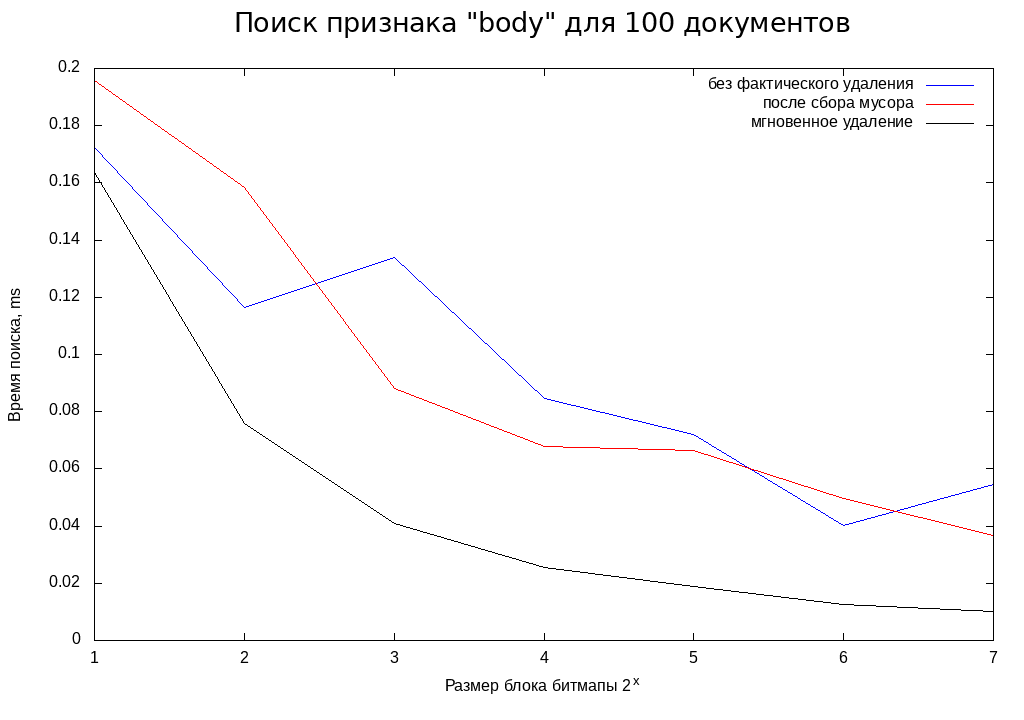
\includegraphics[width=\linewidth, height=10cm]{fig/limit_1e6/1e2/body_time.png}
\caption{Признак \textit{body} встречается в 21\% документов}
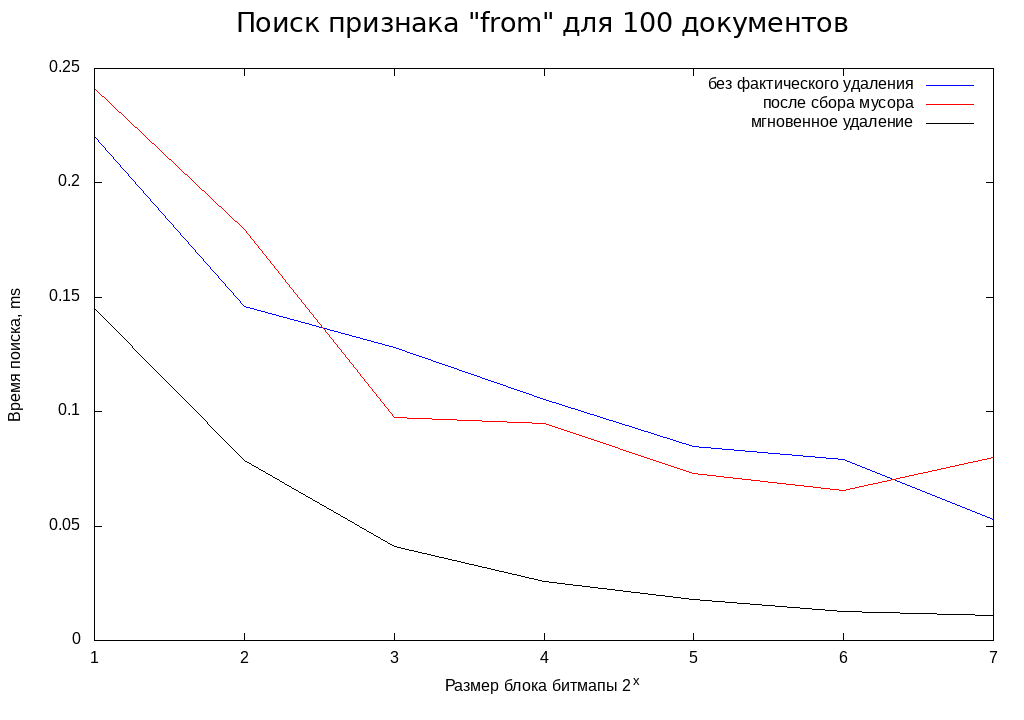
\includegraphics[width=\linewidth, height=11cm]{fig/limit_1e6/1e2/from_time.png}
\caption{Признак \textit{from} встречается в 34\% документов}
\end{figure}

\begin{figure}[H]
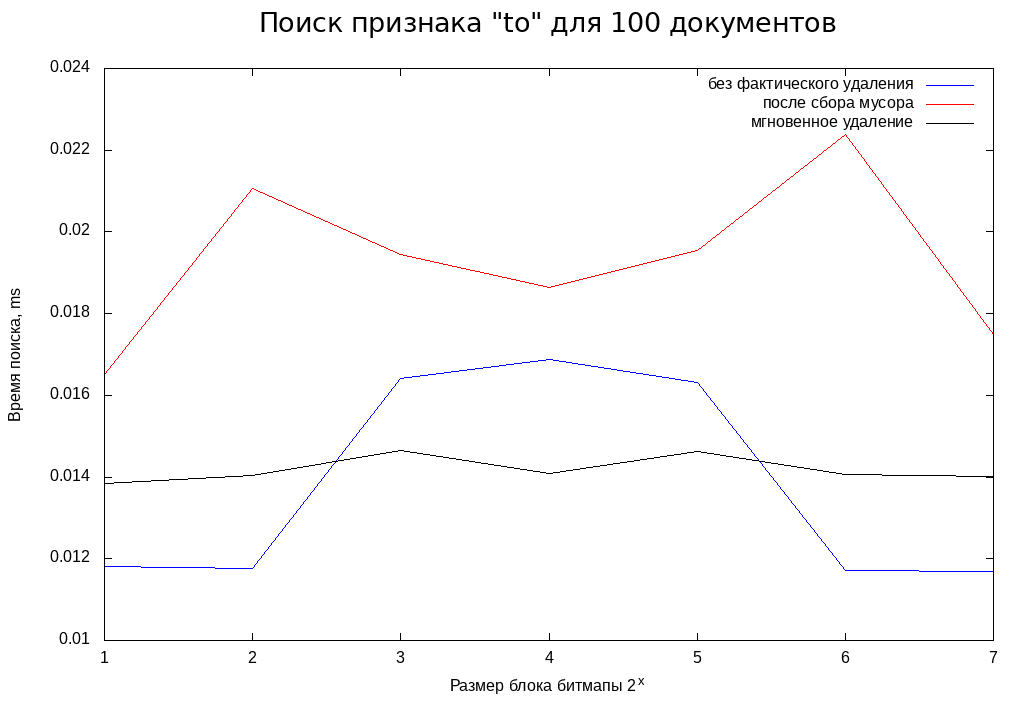
\includegraphics[width=\linewidth, height=11cm]{fig/limit_1e6/1e2/to_time.png}
\caption{Признак \textit{to} встречается в 1\% документов}
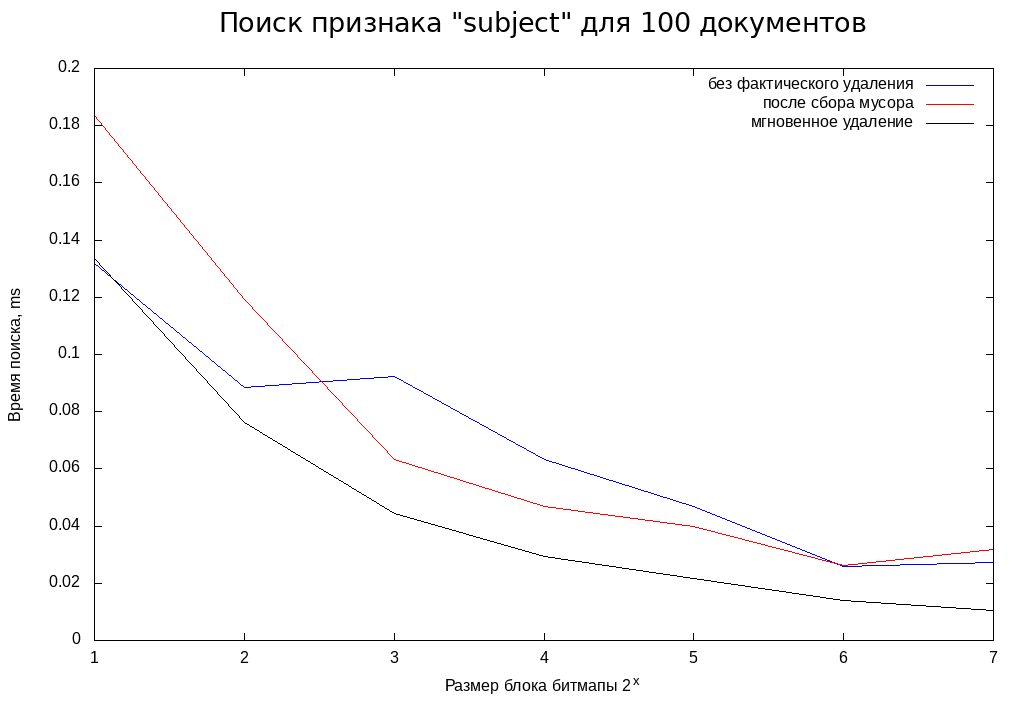
\includegraphics[width=\linewidth, height=11cm]{fig/limit_1e6/1e2/subject_time.png}
\caption{Признак \textit{subject} встречается в 9\% документов}
\end{figure}

\textbf{Вывод}: для 100 элементов алгоритм <<мновенного>> удаления
эффективнее сбора мусора.

\subsubsection{Добавление $10^3$ документов}

\begin{figure}[H]
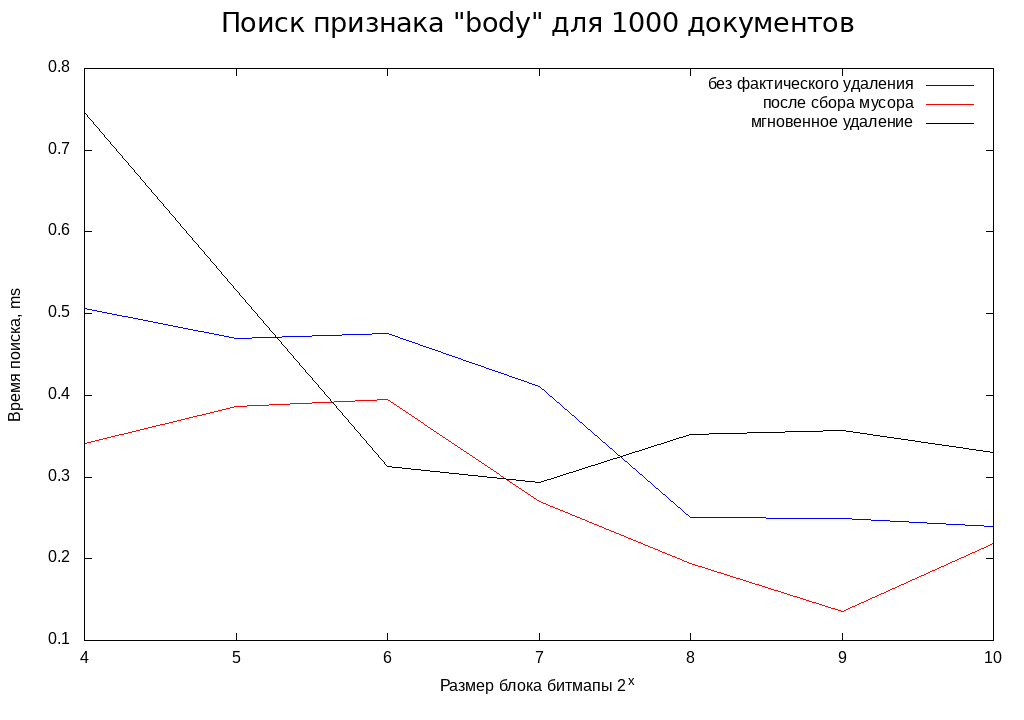
\includegraphics[width=\linewidth, height=10cm]{fig/limit_1e6/1e3/body_time.png}
\caption{Признак \textit{body} встречается в 16\% документов}
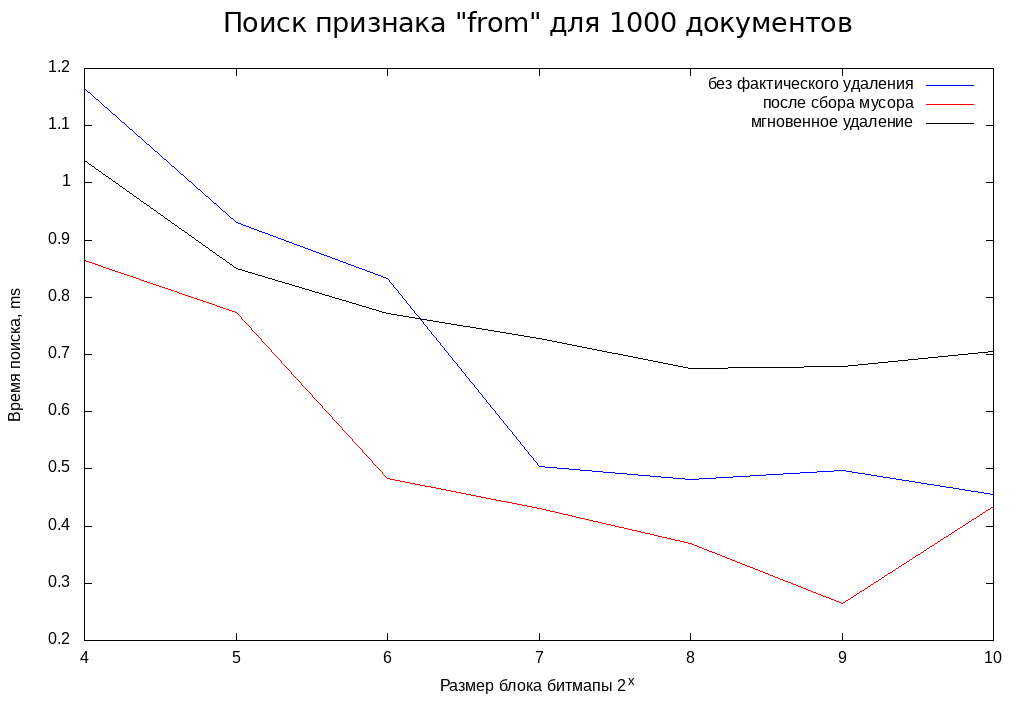
\includegraphics[width=\linewidth, height=11cm]{fig/limit_1e6/1e3/from_time.png}
\caption{Признак \textit{from} встречается в 31\% документов}
\end{figure}

\begin{figure}[H]
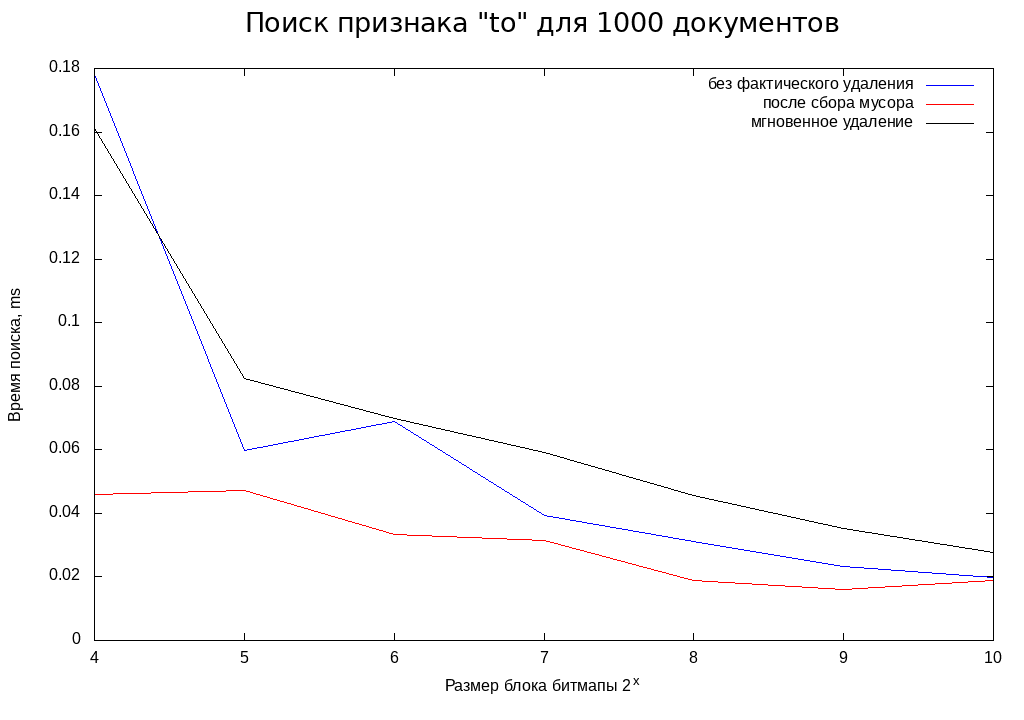
\includegraphics[width=\linewidth, height=11cm]{fig/limit_1e6/1e3/to_time.png}
\caption{Признак \textit{to} встречается менее, чем в 1\% документов}
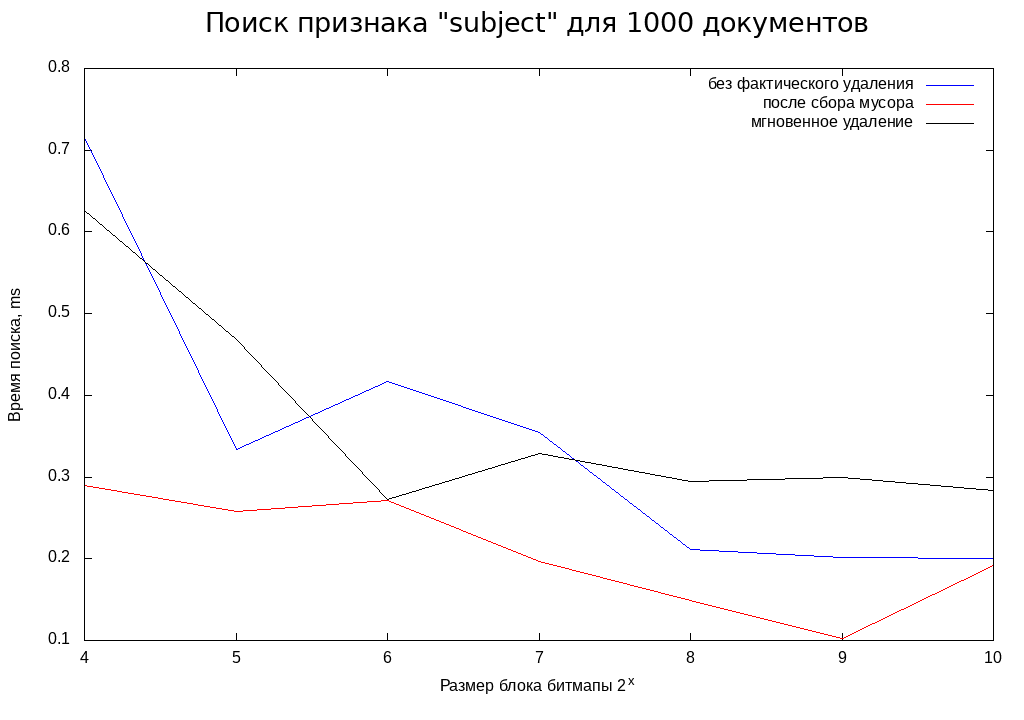
\includegraphics[width=\linewidth, height=11cm]{fig/limit_1e6/1e3/subject_time.png}
\caption{Признак \textit{subject} встречается в 13\% документов}
\end{figure}

\textbf{Вывод}: для 1000 элементов алгоритм сбора мусора дает существенный
прирост в скорости поиска по сравнению с <<мгновенным>> удалением и поиском в данных с мусором.

\subsubsection{Добавление $10^4$ документов}

\begin{figure}[H]
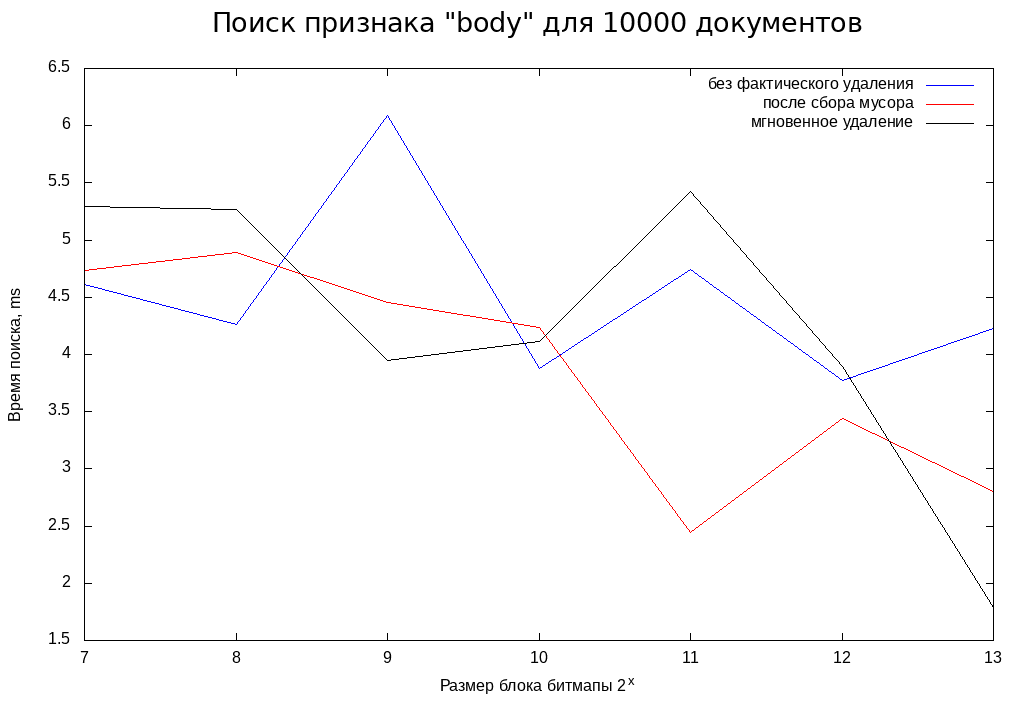
\includegraphics[width=\linewidth, height=10cm]{fig/limit_1e6/1e4/body_time.png}
\caption{Признак \textit{body} встречается в 18\% документов}
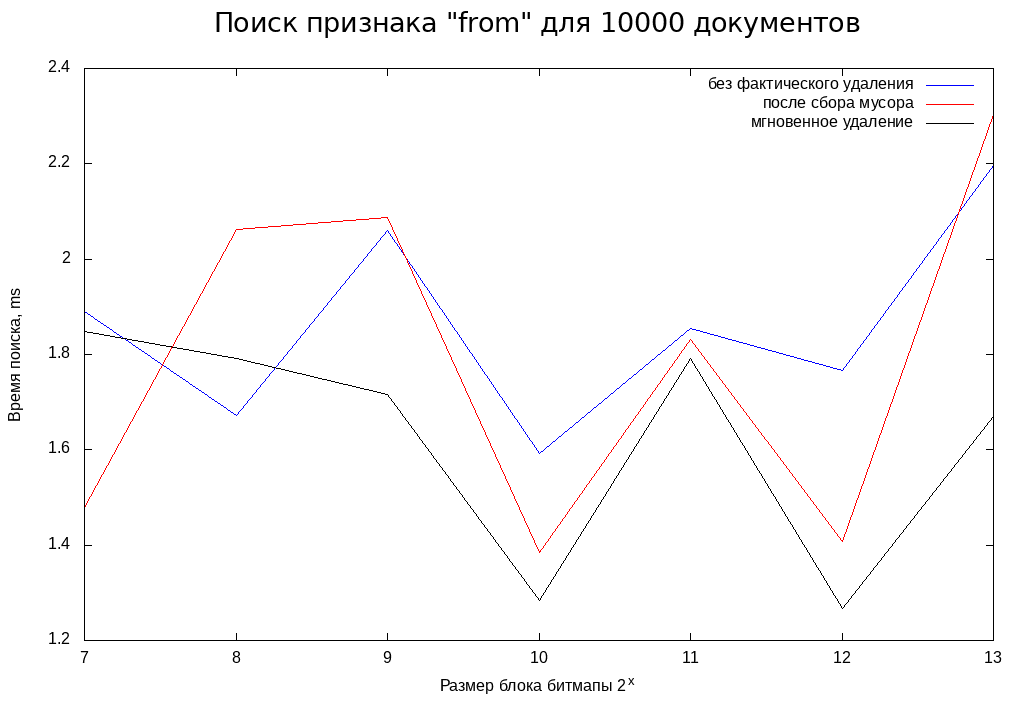
\includegraphics[width=\linewidth, height=11cm]{fig/limit_1e6/1e4/from_time.png}
\caption{Признак \textit{from} встречается в 7\% документов}
\end{figure}

\begin{figure}[H]
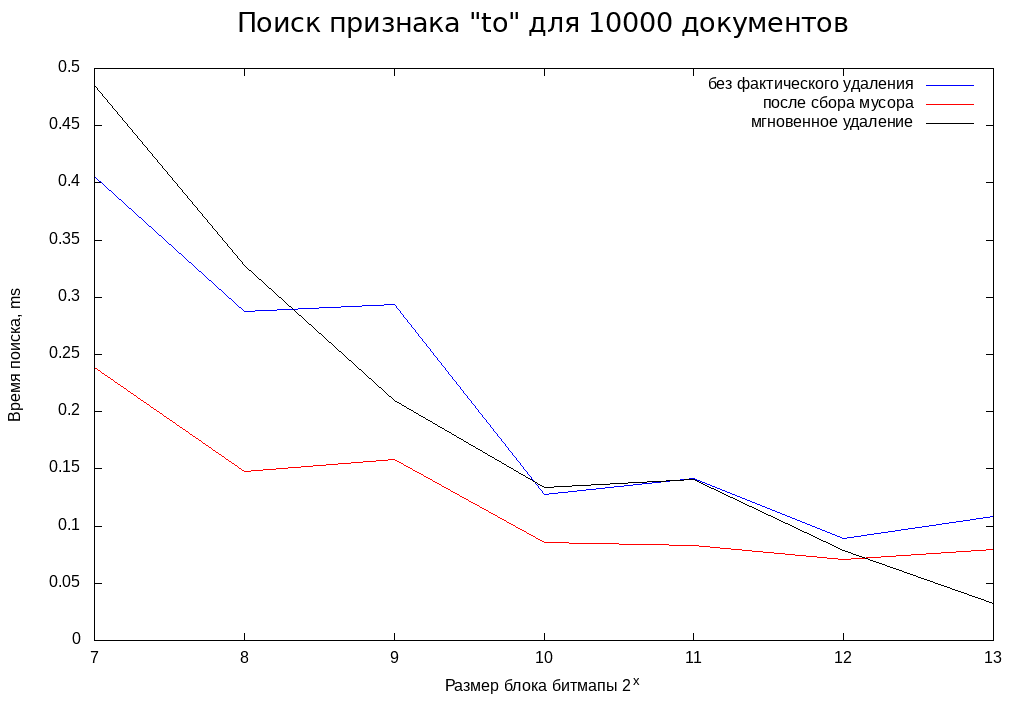
\includegraphics[width=\linewidth, height=11cm]{fig/limit_1e6/1e4/to_time.png}
\caption{Признак \textit{to} встречается менее, чем в 1\% документов}
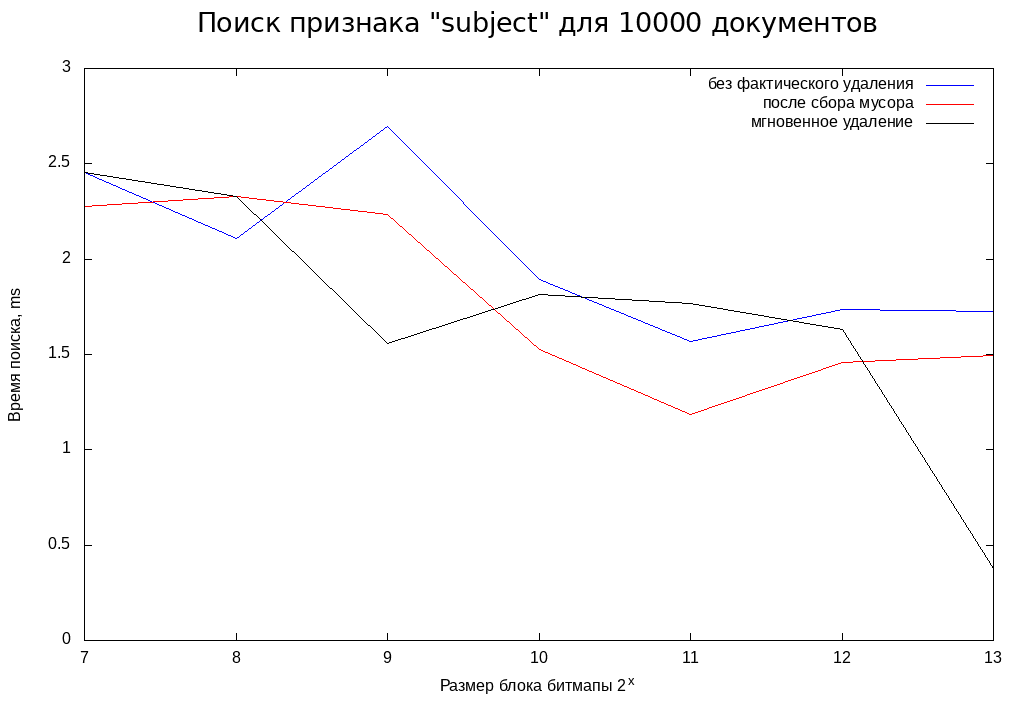
\includegraphics[width=\linewidth, height=11cm]{fig/limit_1e6/1e4/subject_time.png}
\caption{Признак \textit{subject} встречается в 8\% документов}
\end{figure}

\textbf{Вывод}: для $10^4$ элементов алгоритм сбора мусора дает выигрыш на большинстве признаков
по сравнению в <<мгновенным>> удалением и поиском в данных с мусором.

\subsubsection{Добавление $10^5$ документов}

\begin{figure}[H]
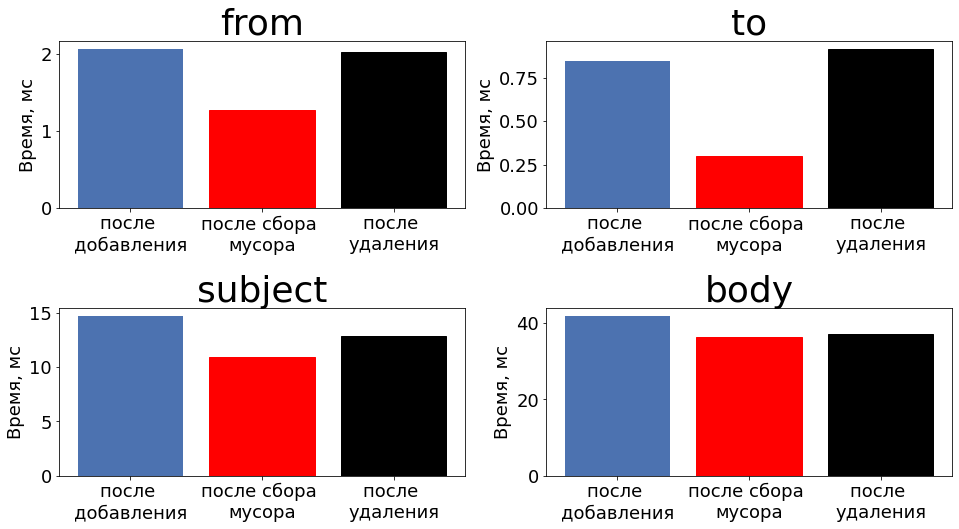
\includegraphics[width=\linewidth]{fig/limit_1e6/1e5/search.png}
\caption{Размер блока $2^{10}$}
\end{figure}

\textbf{Вывод}: для $10^5$ добавленных документов алгоритм сбора мусора эффективнее
по сравнению в <<мгновенным>> удалением и поиском в данных с мусором.

\newpage
\subsection{Поисковый запрос по первому вхождению заданного ключа для фиксированного числа добавленных элементов}

\subsubsection{Добавление $10^2$ документов}

\begin{figure}[H]
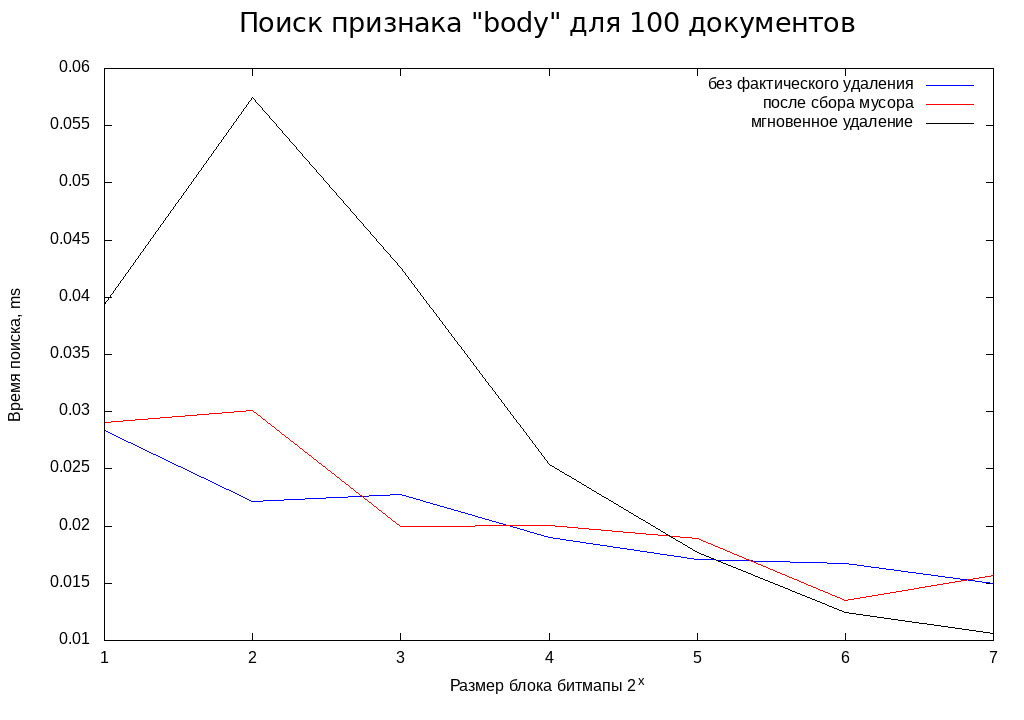
\includegraphics[width=\linewidth, height=10cm]{fig/limit_1/1e2/body_time.png}
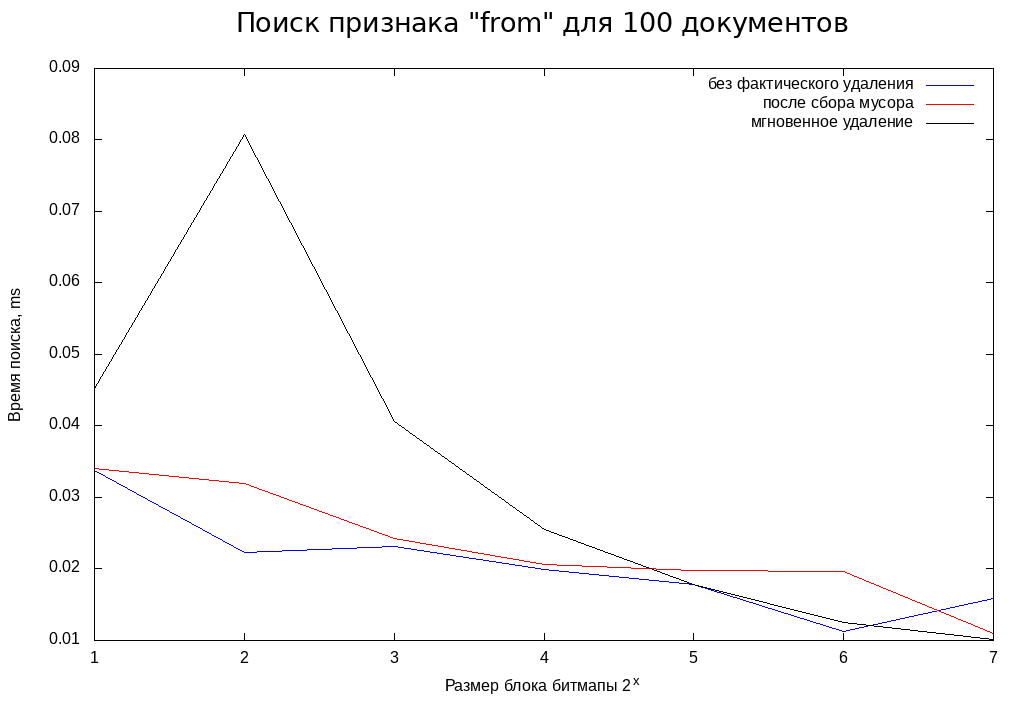
\includegraphics[width=\linewidth, height=11cm]{fig/limit_1/1e2/from_time.png}
\end{figure}

\begin{figure}[H]
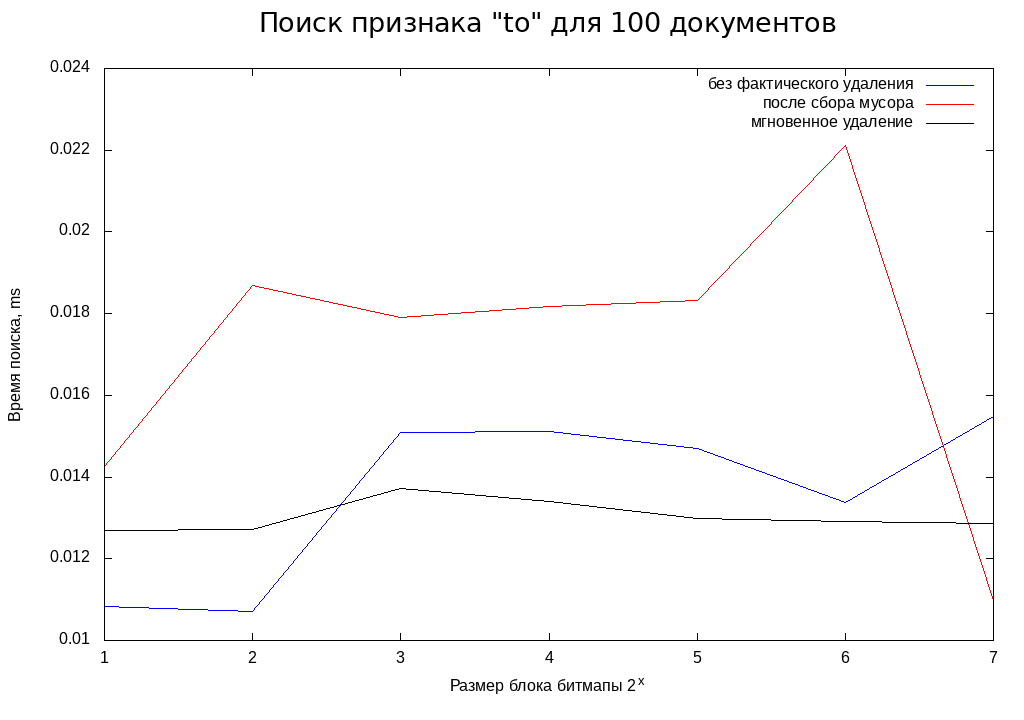
\includegraphics[width=\linewidth, height=11cm]{fig/limit_1/1e2/to_time.png}
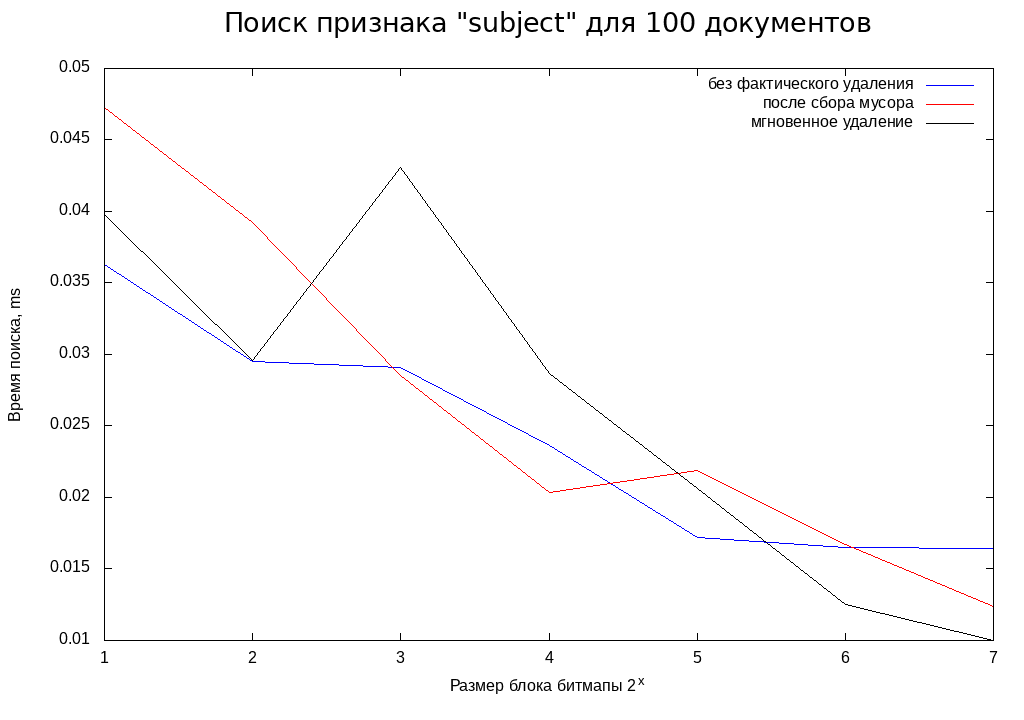
\includegraphics[width=\linewidth, height=11cm]{fig/limit_1/1e2/subject_time.png}
\end{figure}

\textbf{Вывод}: для 100 элементов алгоритм <<мновенного>> удаления и сбора мусора
не вносят существенный вклад в эффективность поиска единственного ключа.

\subsubsection{Добавление $10^3$ документов}

\begin{figure}[H]
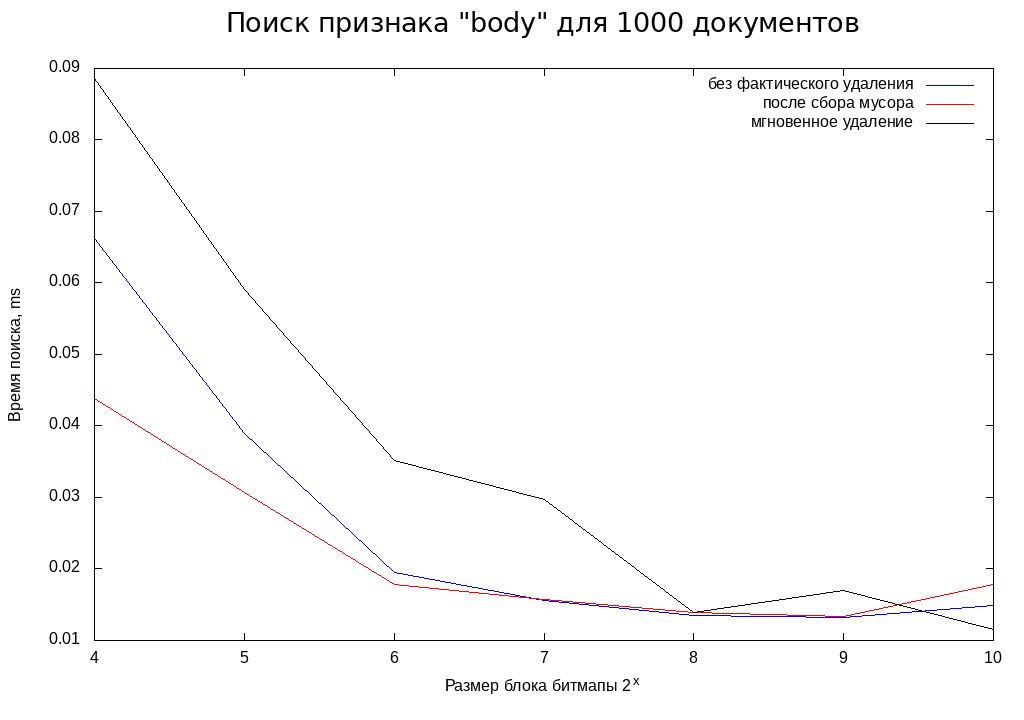
\includegraphics[width=\linewidth, height=10cm]{fig/limit_1/1e3/body_time.png}
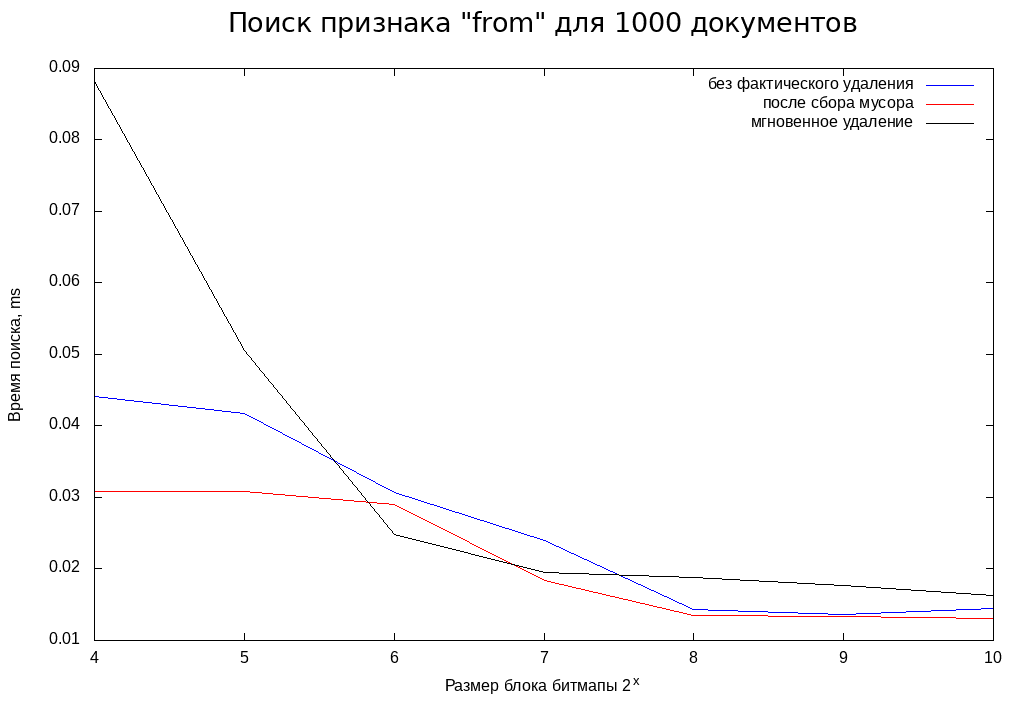
\includegraphics[width=\linewidth, height=11cm]{fig/limit_1/1e3/from_time.png}
\end{figure}

\begin{figure}[H]
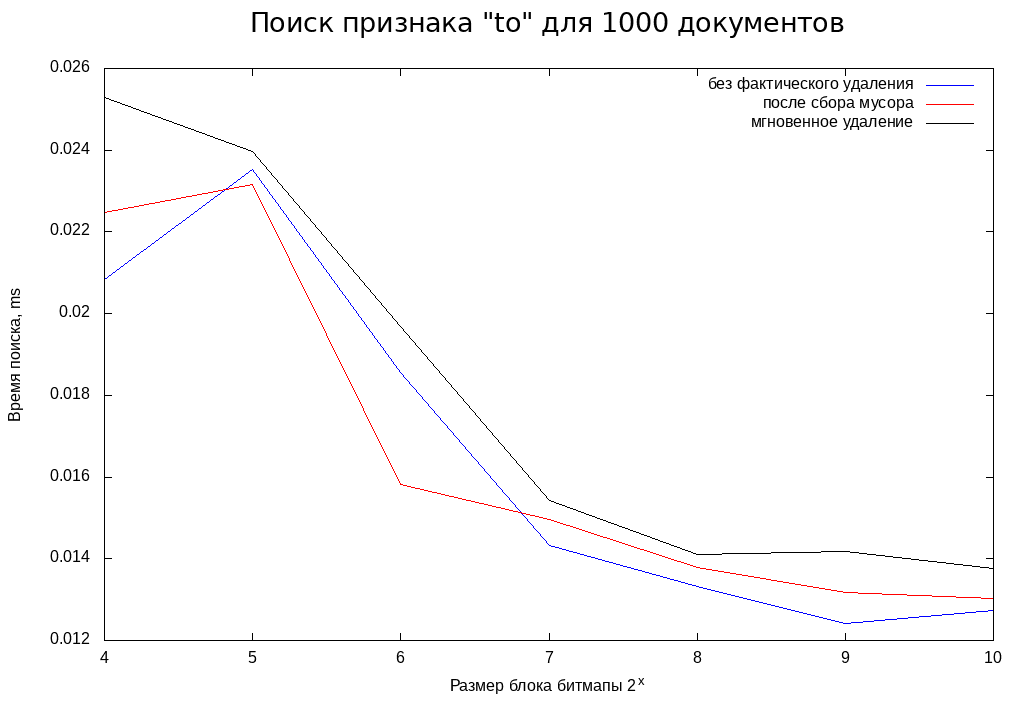
\includegraphics[width=\linewidth, height=11cm]{fig/limit_1/1e3/to_time.png}
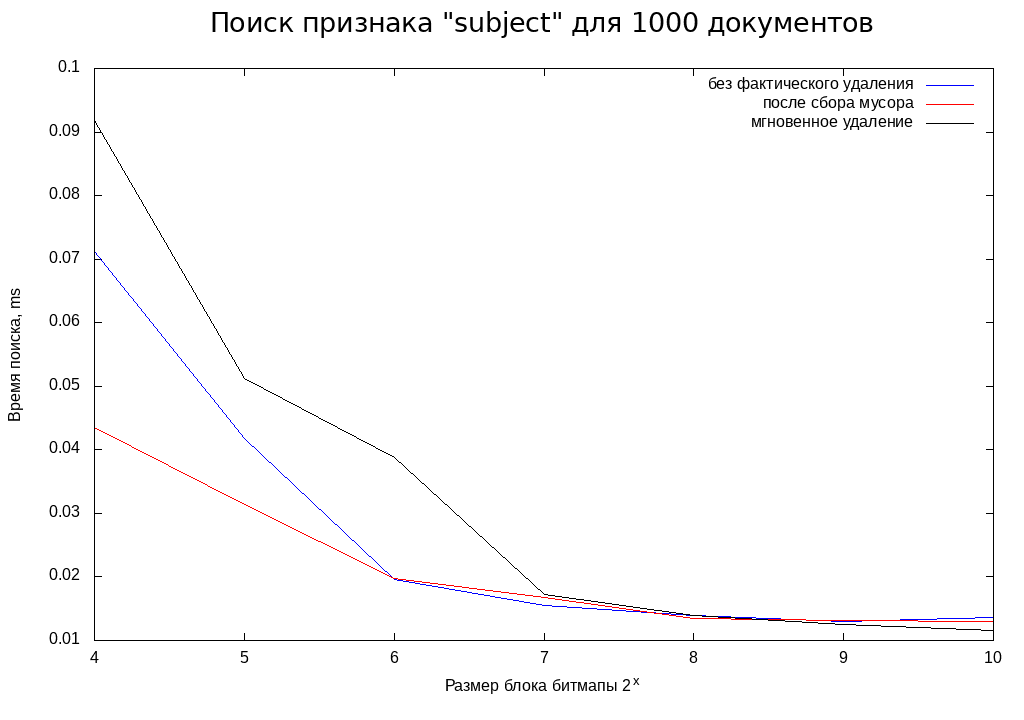
\includegraphics[width=\linewidth, height=11cm]{fig/limit_1/1e3/subject_time.png}
\end{figure}

\textbf{Вывод}: для 1000 элементов алгоритм <<мновенного>> удаления и сбора мусора
не вносят существенный вклад в эффективность поиска единственного ключа.

\subsubsection{Добавление $10^4$ документов}

\begin{figure}[H]
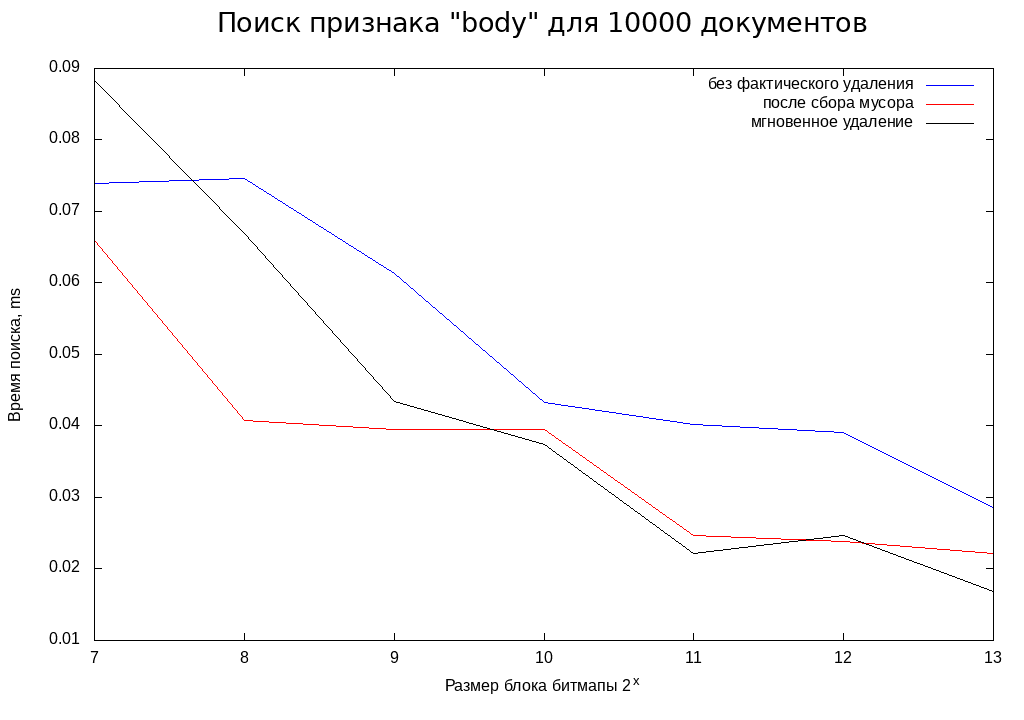
\includegraphics[width=\linewidth, height=10cm]{fig/limit_1/1e4/body_time.png}
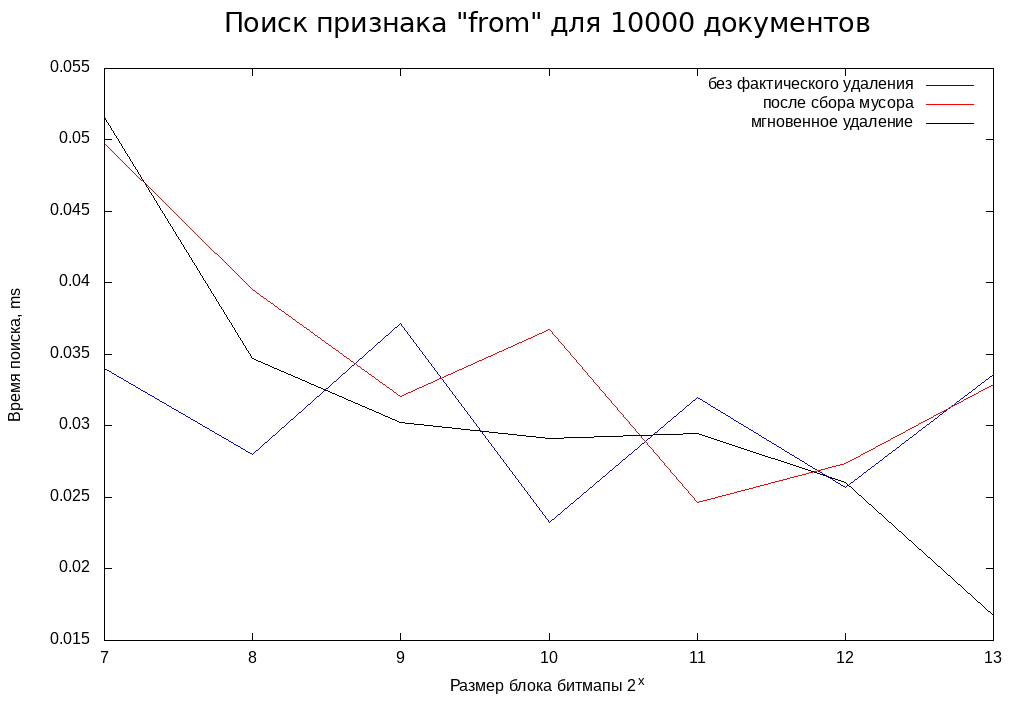
\includegraphics[width=\linewidth, height=11cm]{fig/limit_1/1e4/from_time.png}
\end{figure}

\begin{figure}[H]
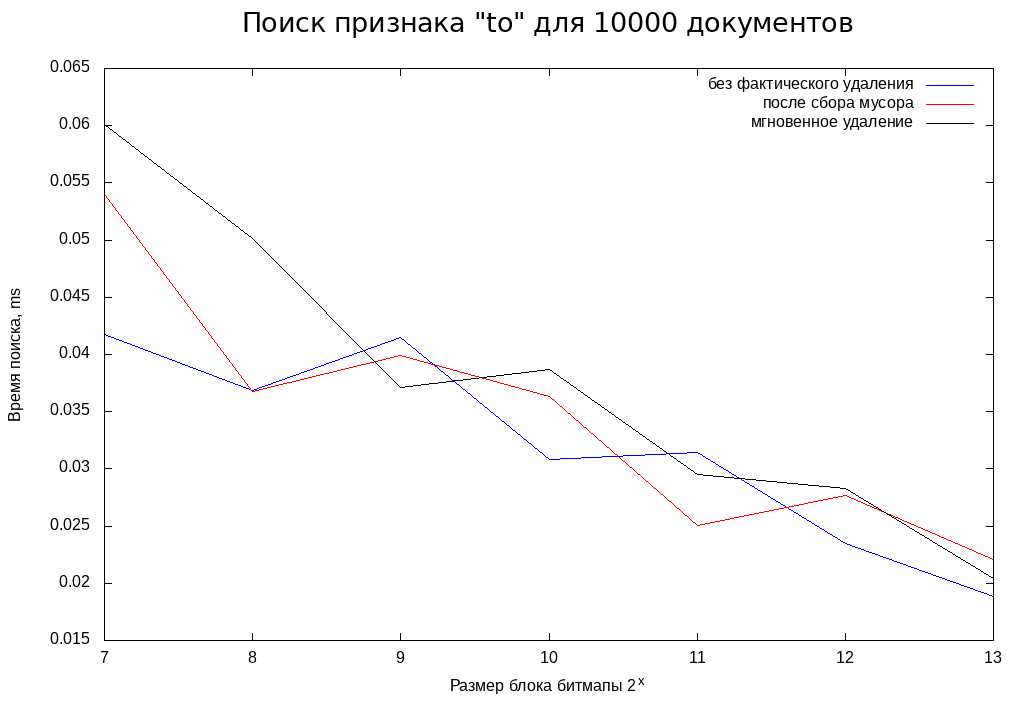
\includegraphics[width=\linewidth, height=11cm]{fig/limit_1/1e4/to_time.png}
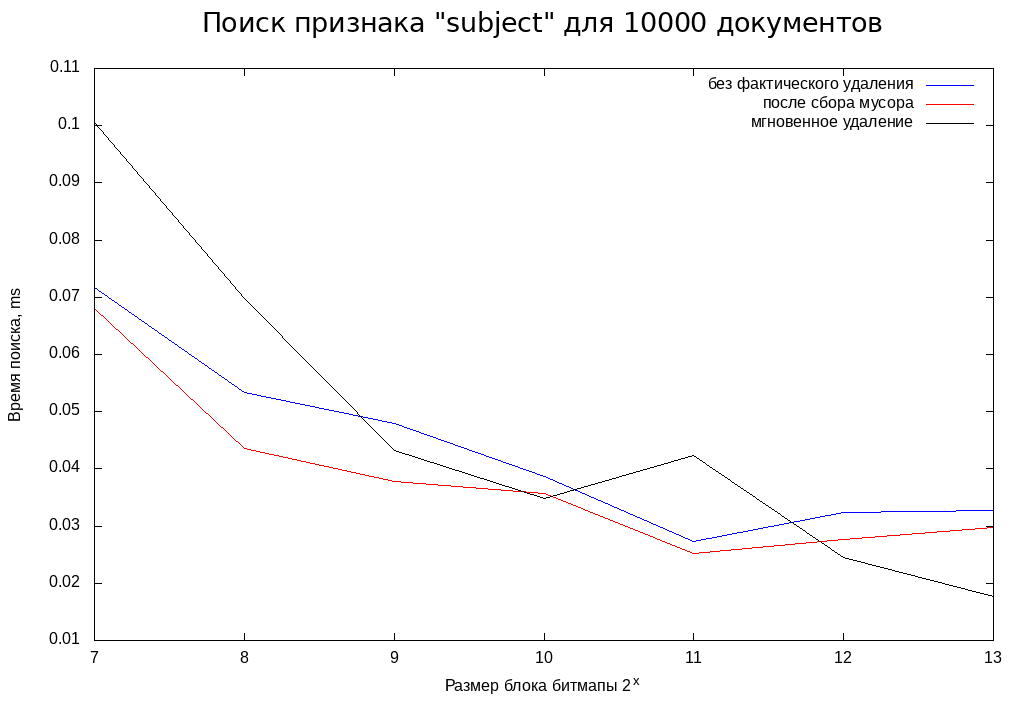
\includegraphics[width=\linewidth, height=11cm]{fig/limit_1/1e4/subject_time.png}
\end{figure}

\textbf{Вывод}: для $10^4$ элементов алгоритм сбора мусора дает выигрыш на большинстве признаков
по сравнению в <<мгновенным>> удалением и поиском в данных с мусором.

\subsubsection{Добавление $10^5$ документов}

\begin{figure}[H]
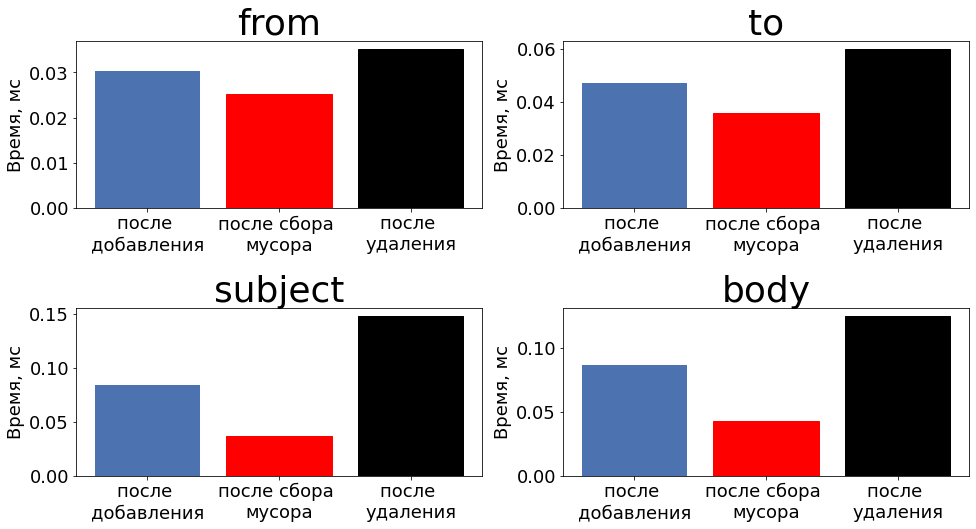
\includegraphics[width=\linewidth]{fig/limit_1/1e5/search.png}
\caption{Размер блока $2^{10}$}
\end{figure}

\textbf{Вывод}: для $10^5$ добавленных документов алгоритм сбора мусора эффективнее
по сравнению в <<мгновенным>> удалением и поиском в данных с мусором.

\newpage
\subsection{Сравнение времени работы алгоритмов для различного числа добавленных документов}

\subsubsection{Добавление $10^2$ документов, удаление $\frac{2}{3}$ документов}

\begin{figure}[H]
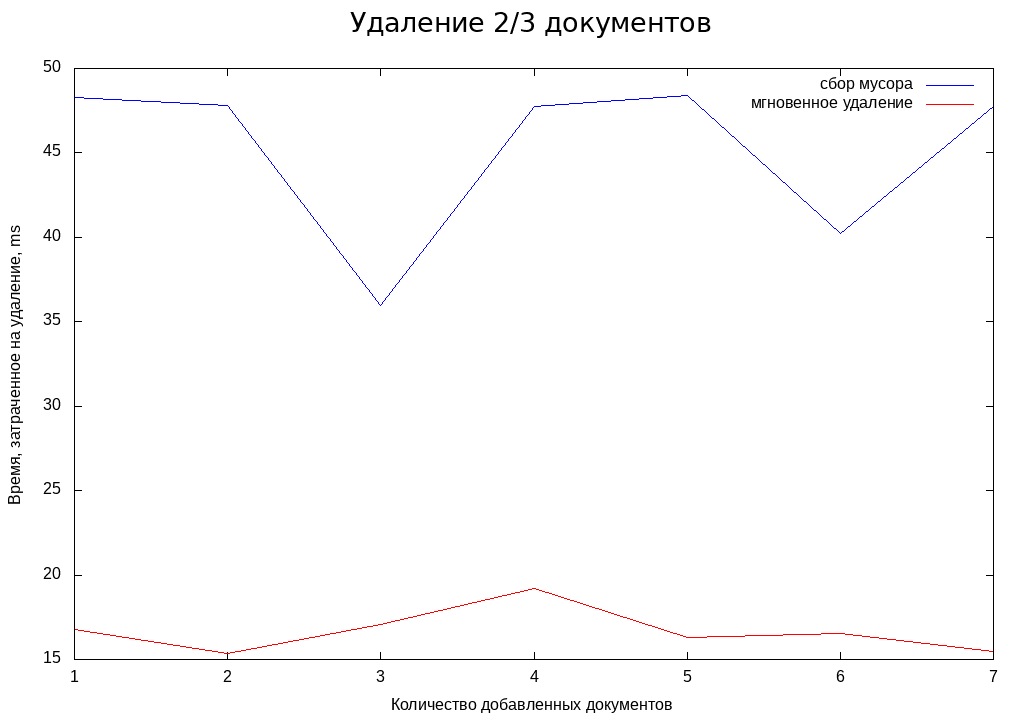
\includegraphics[width=\linewidth, height=10cm]{fig/time_1e2.png}
\end{figure}

\subsubsection{Добавление $10^3$ документов, удаление $\frac{2}{3}$ документов}
\begin{figure}[H]
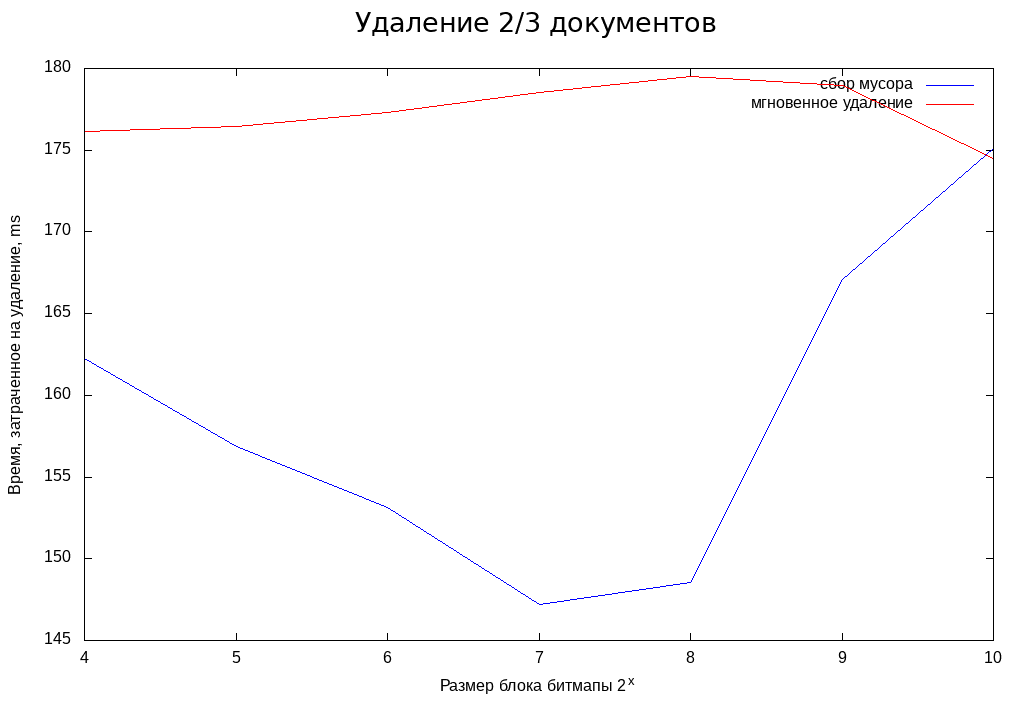
\includegraphics[width=\linewidth, height=10cm]{fig/time_1e3.png}
\end{figure}

\textbf{Вывод}: для 100 элементов алгоритм <<мновенного>> удаления
эффективнее сбора мусора. Получается, что для малого числа документов использование
отложенного удаления вида сбора мусора нелогично. Для 1000 элементов алгоритм
<<мновенного>> удаления медленнее алгоритма сбора мусора.

\subsubsection{Добавление $10^4$ документов, удаление $\frac{2}{3}$ документов}
\begin{figure}[H]
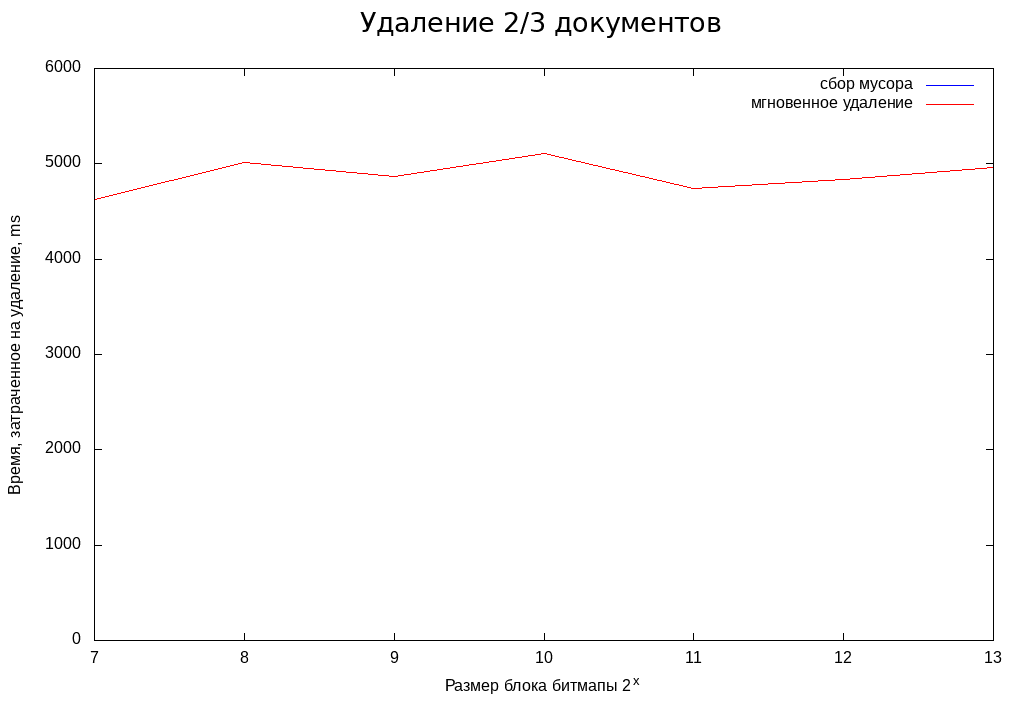
\includegraphics[width=\linewidth, height=11cm]{fig/time_1e4.png}
\end{figure}

\begin{table}[H]
      \caption{Время работы алгоритмов для $10^4$ документов, мс}
      \centering
      \small
      \singlespacing
      \begin{tabular}{|c|c|c|}
            \hline
            Размер блока & Сбор мусора                & <<Мгновенное удаление>> \\ \hline \hline
            7            & 0.269618                   & 4627.649                \\ \hline
            8            & 0.272035                   & 5012.865                \\ \hline
            9            & 0.276679                   & 4864.4414               \\ \hline
            10           & 0.254468                   & 5110.06                 \\ \hline
            11           & 0.25441                    & 4744.915                \\ \hline
            12           & 0.254357                   & 4838.297                \\ \hline
            13           & 0.25433                    & 4966.4146               \\ \hline
\end{tabular}
\end{table}

\textbf{Вывод}: для $10^4$ документов алгоритм становится в тысячи раз
эффективнее метода в лоб: <<мгновенного удаления>>.

\subsubsection{Добавление $10^5$ документов, удаление $\frac{2}{3}$ документов}
\begin{figure}[H]
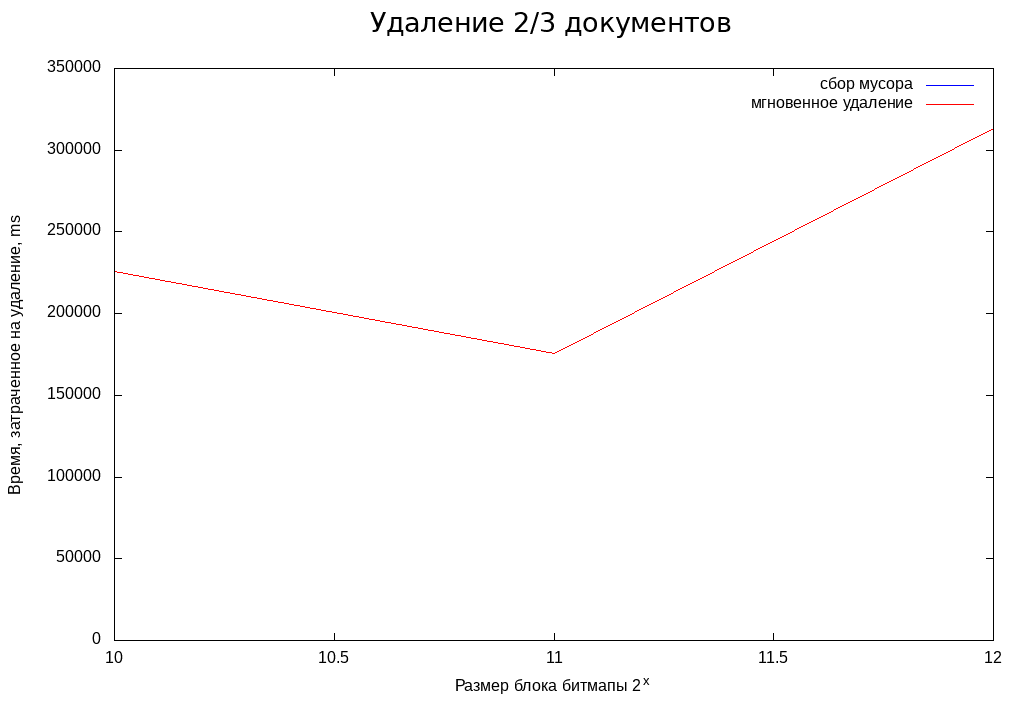
\includegraphics[width=\linewidth, height=11cm]{fig/time_1e5.png}
\end{figure}

\begin{table}[H]
      \caption{Время работы алгоритмов для $10^5$ документов, мс}
      \centering
      \small
      \singlespacing
      \begin{tabular}{|c|c|c|}
            \hline
            Размер блока & Сбор мусора                & <<Мгновенное удаление>> \\ \hline \hline
            10           & 0.253822                   & 225616.848              \\ \hline
            11           & 0.254688                   & 175847.244              \\ \hline
            12           & 0.254053                   & 313510.579              \\ \hline
\end{tabular}
\end{table}

\textbf{Вывод}: для $10^5$ документов алгоритм становится в тысячи раз
эффективнее метода в лоб: <<мгновенного удаления>>.

\newpage
\subsection{Статистика количества операций записи, чтения и слияния для различного числа добавленных документов}

Во время выполнения тестов производительности на поиск элементов мы замеряли
некоторые статистические показатели: количество обращений в долгосрочную память
на жестком диске (операций чтения и записи), количество слияний с данными на
диске.
\subsubsection{Количество операций записи на диск}

\begin{figure}[H]
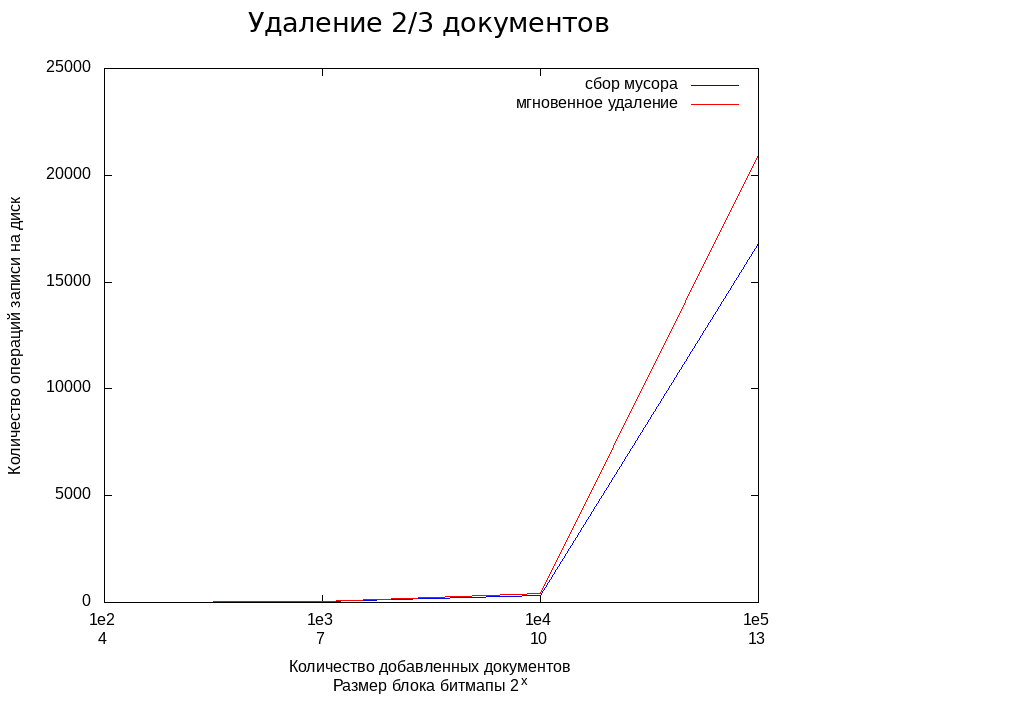
\includegraphics[width=\linewidth]{fig/writecalls.png}
\end{figure}

\begin{table}[H]
      \caption{Количество операций записи на диск}
      \centering
      \small
      \singlespacing
      \begin{tabular}{|c|c|c|}
            \hline
            Количество добавленных документов   & Сбор мусора                 & <<Мгновенное удаление>>     \\ \hline \hline
            100                                 & 8                           & 9                           \\ \hline
            1000                                & 38                          & 46                          \\ \hline
            10000                               & 347                         & 413                         \\ \hline
            100000                              & 16791                       & 20967                       \\ \hline
\end{tabular}
\end{table}

\subsubsection{Количество операций слияния с данными на диске}

\begin{figure}[H]
\centering
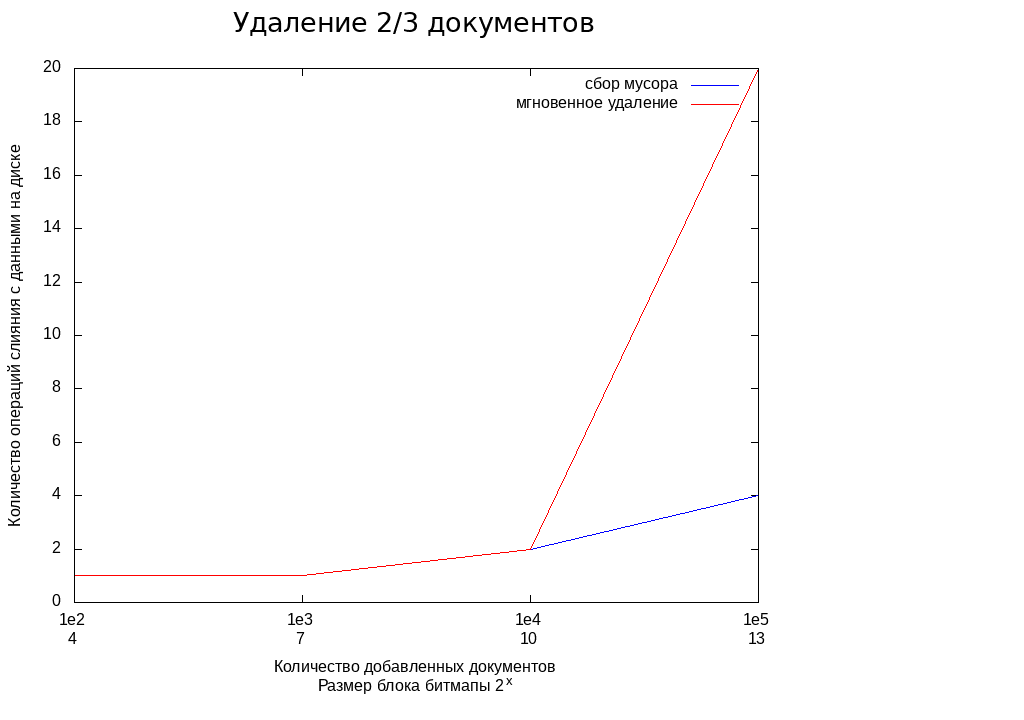
\includegraphics[width=\linewidth]{fig/merges.png}
\end{figure}

\begin{table}[H]
      \caption{Количество операций записи на диск}
      \centering
      \small
      \singlespacing
      \begin{tabular}{|c|c|c|}
            \hline
            Количество добавленных документов   & Сбор мусора                 & <<Мгновенное удаление>>     \\ \hline \hline
            100                                 & 1                           & 1                           \\ \hline
            1000                                & 1                           & 1                           \\ \hline
            10000                               & 2                           & 2                           \\ \hline
            100000                              & 4                           & 20                          \\ \hline
\end{tabular}
\end{table}

\textbf{Вывод}: алгоритм сбора мусора оказывается эффективнее в плане
обращений к <<медленной>> памяти по всем метрикам при увеличении размера 
обрабатываемых данных.

%\newpage
\section{Выводы}

Алгоритм сбора мусора оправдал теоретические ожидания эффективности времени
поиска и длительности исполнения по сравнению с алгоритмом <<мгновенного>>
удаления. 

Время поиска по всем вхождения ключа при фиксированном количестве
добавленных документов и размере блока дает выигрыш по сравнению
с поиском в индексе с мусором и алгоритмом <<мгновенного>> удаления при числе
добавленных документов $N \ge 10^3$. Данный результат получается для большинства
признаков с различной частотой встречаемости в документах.

Время поиска по первому вхождению ключа при фиксированном количестве
добавленных документов и размере блока не дает существенного выигрыша по
сравнению с поиском в индексе с мусором и алгоритмом <<мгновенного>> удаления
при числе добавленных документов $N \leq 10^5$. Данный результат логичен с точки
зрения устройства индекса.

Кроме того, наблюдается кратный выигрыш в скорости выполнения алгоритма сбора
мусора. Время работы выходит на линейный рост с малым наклоном при увеличении
числа документов $N$ в то время как алгоритм <<мгновенного>> удаления растет
экспоненциально.

В то же время предлагаемый метод не лишён важных недостатков. Хотя индекс,
построенный по этому принципу, и позволяет производить эффективный поиск по
всем вхождениям ключа, существенный разрыв с простым подходом проявляется лишь
при большом числе добавленных документов. Это соответствует реальным требованиями
к поисковым системам. Это также значит, что в случае, когда возможна реализация
случаев работы с малым числом данных, необходимо комбинировать два подхода для
различных целей.

%\newpage
\section{Заключение}

В работе проанализированы существующие подходы к сбору данных в базах данных
и поисковых системах, т.~е. эффективному и своевременному удалению объектов,
потерявших актуальность и/или указывающих на несуществующие документы.
Предложен подход к решению этой задачи --- периодический сбор мусора в блоках
данных при превышении числа удаленных документов порогового значения,
позволяющий добиться хорошей производительности запросов по вхождениям
ключа при фиксированном количестве добавленных и удаленных документов. Рассмотрено поведение
предлагаемого алгоритма в сравнении с известными подходами для некоторых
сценариев использования, и показано экспериментально, что
даже при большом количестве добавленных документов ($\ge 10^{4}$)
предложенный алгоритм дает выигрыш во времени поиска. Также
простой подход дает экспоненциальный рост времени выполнения от количества
документов, а в случае разработанного алгоритма это время практически
не растёт.

Получена теоретическая оценка размеров дополнительной памяти для реализации
обоих подходов в зависимости от количества добавленных и удаленных документов,
разреженности битовых карт и порядка удаления, подтверждённая экспериментально.

Возможными направлениями дальнейшего развития данной темы могли бы
стать разработка оценки приоритетности очистки блоков, в том числе с учётом
общего числа удаленных документов, сравнительный анализ поведения для других
видов LSM-деревьев, получение теоретической оценки размера метаданных при более общих
исходных предположениях (например, при динамическом определении порогового значения
и времени старта алгоритма), а также детальное построение эффективного
параллелизуемого алгоритма.

\newpage
\printbibliography

\end{document}
